	\FloatBarrier \subsection{Protéines}
	Les protéines sont des macromolécules\footnote{Une macromolécule est une \og grosse \fg{} molécule, généralement un polymère ; elle est constituée de plusieurs milliers d'atomes.} que l'on retrouve dans les cellules de tous les organismes vivants. Elles assurent un très grand nombre de fonctions cellulaires (structuration de la cellule, mouvements et divisions cellulaires, communication intercellulaire, transport, par exemple de dioxygène, défense immunitaire) et biochimiques (liaison et fixations de molécules, catalyse de réactions biochimiques, etc.) au sein des cellules et des tissus~\cite{lodish2004molecular}. Elles participent aussi au conditionnement de l'acide désoxyribonucléique (ADN) et à la régulation de l'expression génétique. L'étude de leur fonctionnement est donc essentiel à la compréhension du vivant et de ses processus.
	
	\begin{wrapfigure}{O}{0.5\textwidth} % Capital O makes the figure float, because that's totally intuitive and obvious.
		\centering
		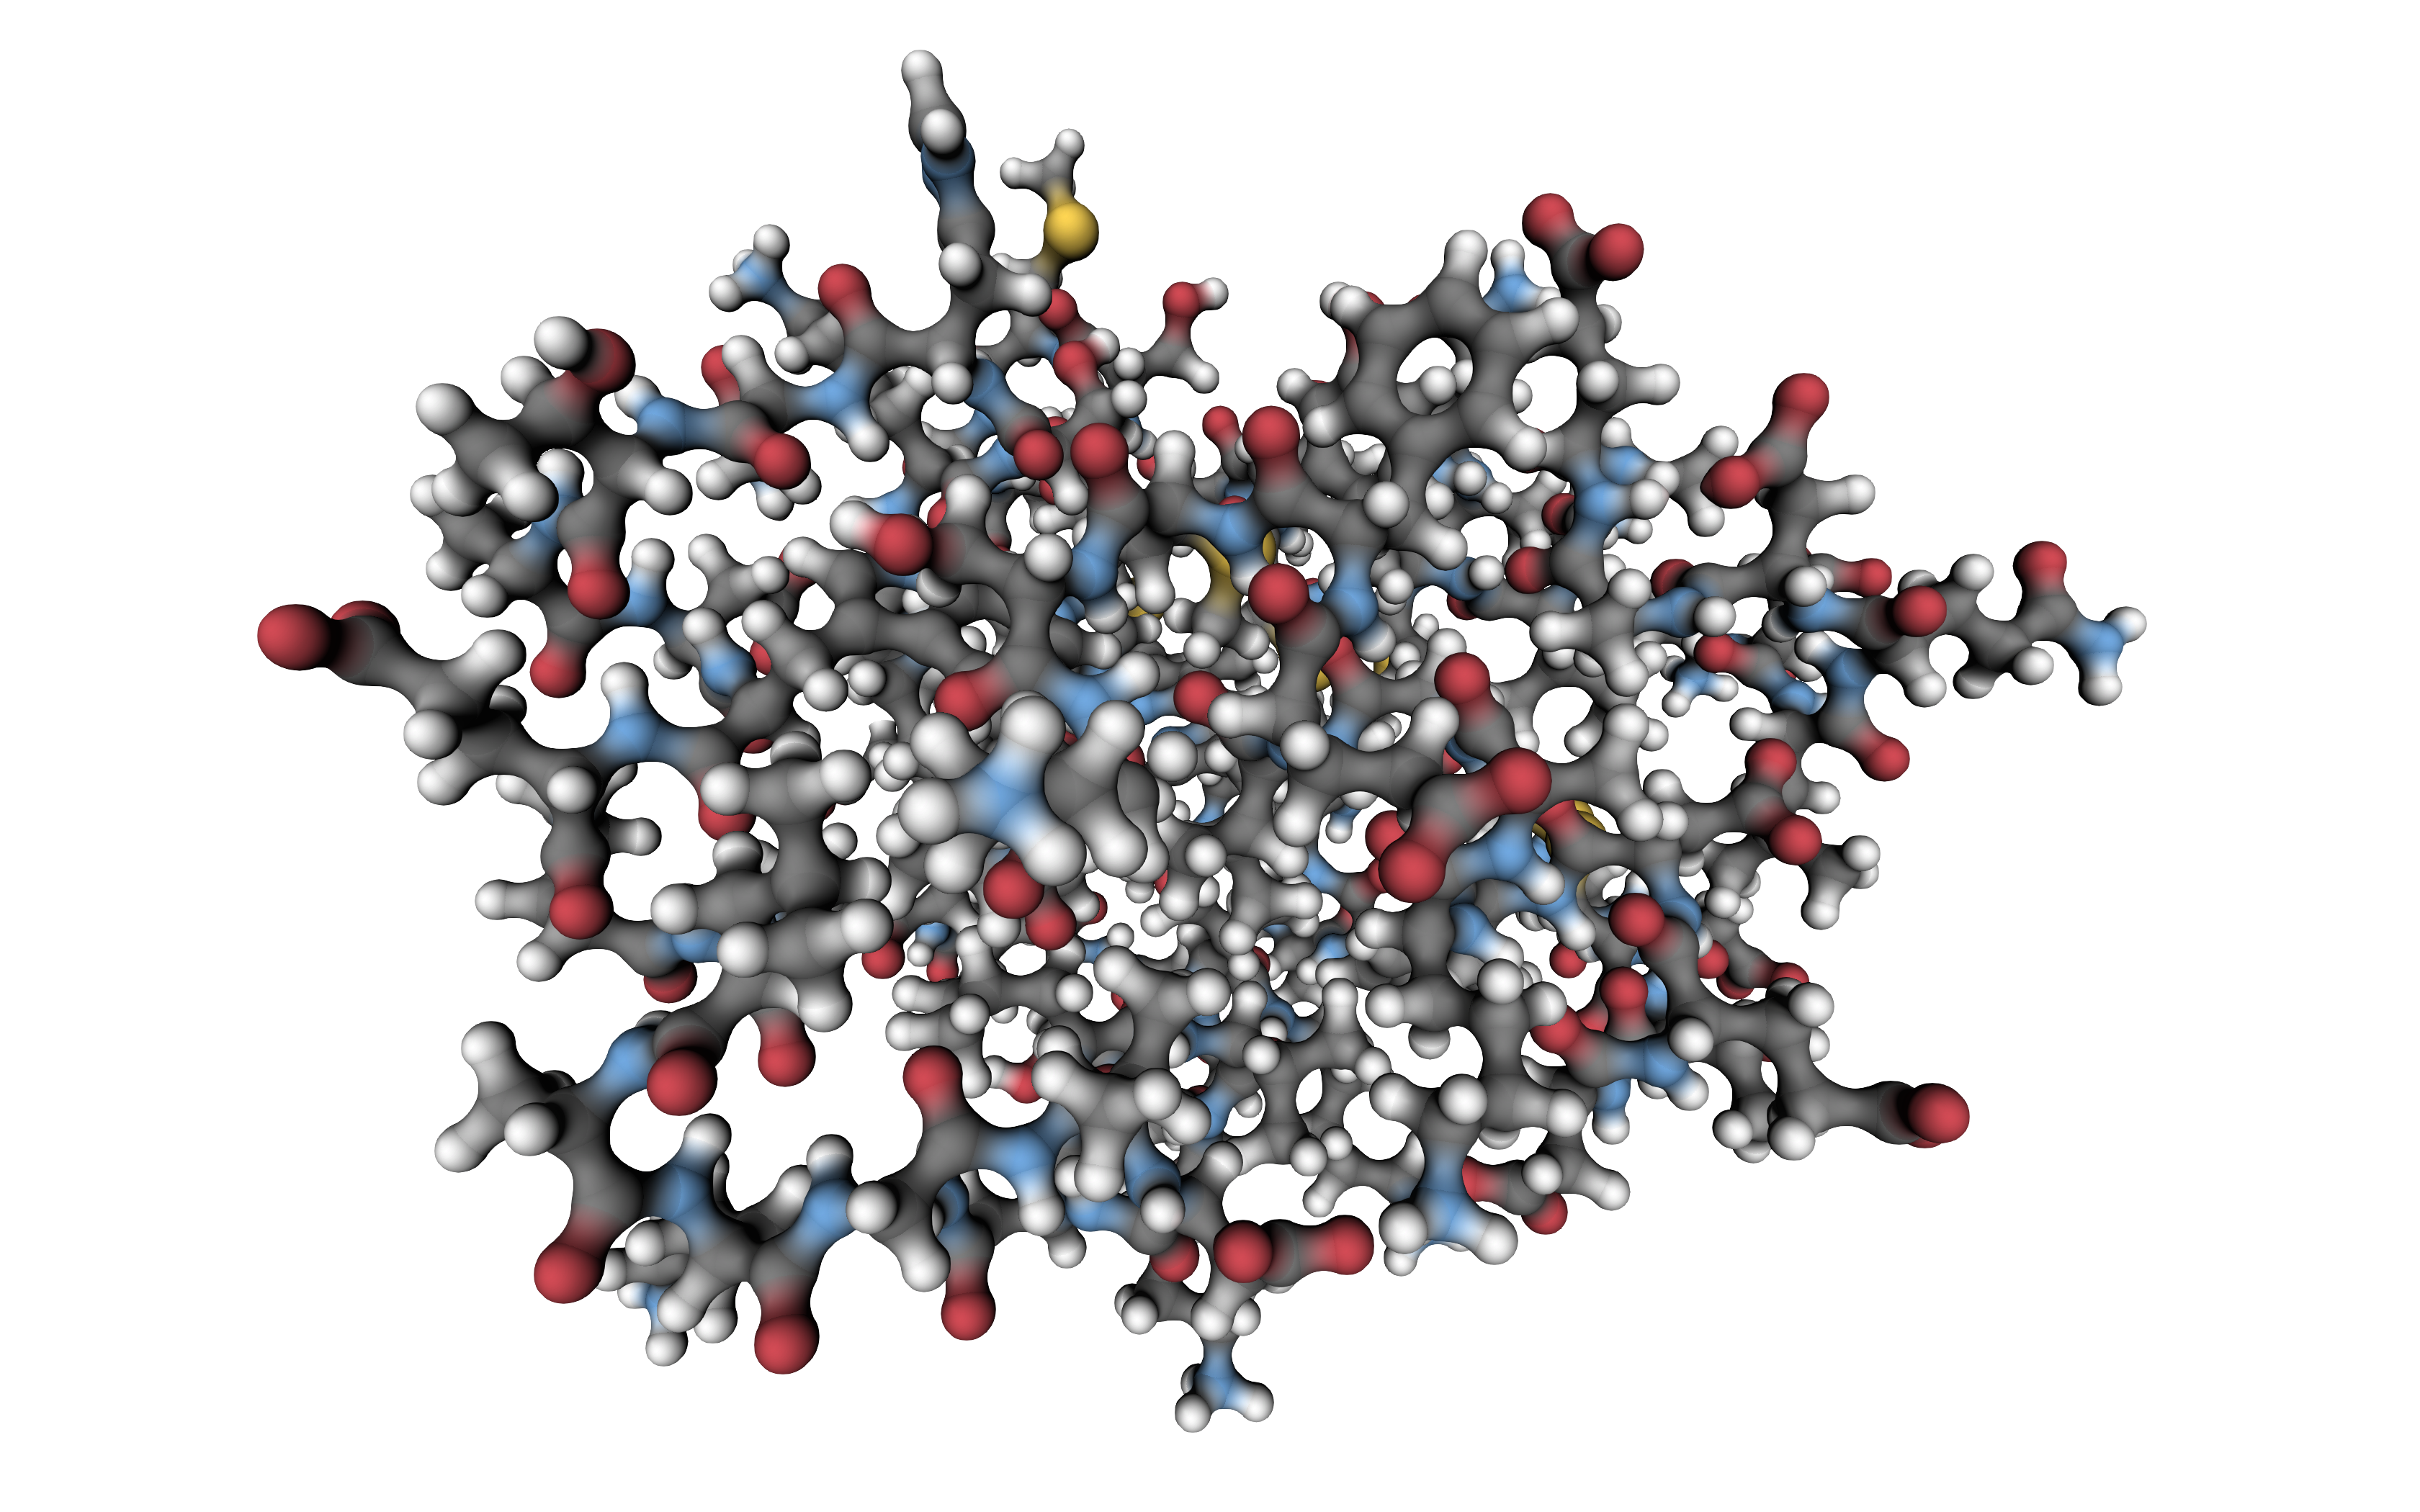
\includegraphics[width=0.46\textwidth]{figures/ch1/1KX2}
		\caption[Une protéine en \emph{Hyperballs}]{Une protéine (\cite{bartalesi2002solution}) représentée avec UnityMol~\cite{doutreligne2014unitymol}. Elle est assez petite (81 acides aminés, vs. $\approx$~30~000 pour la titine), les atomes sont représentés avec un rayon inférieur à leur rayon de vdW, l'occultation est réduite, et les molécules du solvant ne sont pas représentées. Malgré tout, le niveau d'occultation demeure très important.}
		\label{fig:1KX2}
	\end{wrapfigure}
	
	\subsubsection{Composition}
	Concrètement, une protéine est un une  chaîne d'acides aminés, reliés par des liaisons peptidiques, c'est-à-dire des liaisons covalentes entre une fonction carboxyle (–C(O)OH) et une fonction amine (un composé organique dérivé de l'ammoniac dont au moins un atome d'hydrogène a été remplacé par un groupe carboné). Ces chaînes d'acides aminés sont également appelées chaînes polypeptidiques, ou simplement polypeptides.
	
	\begin{figure}[htb]
		%\centering
		\begin{subfigure}{.39\textwidth}
			\centering
			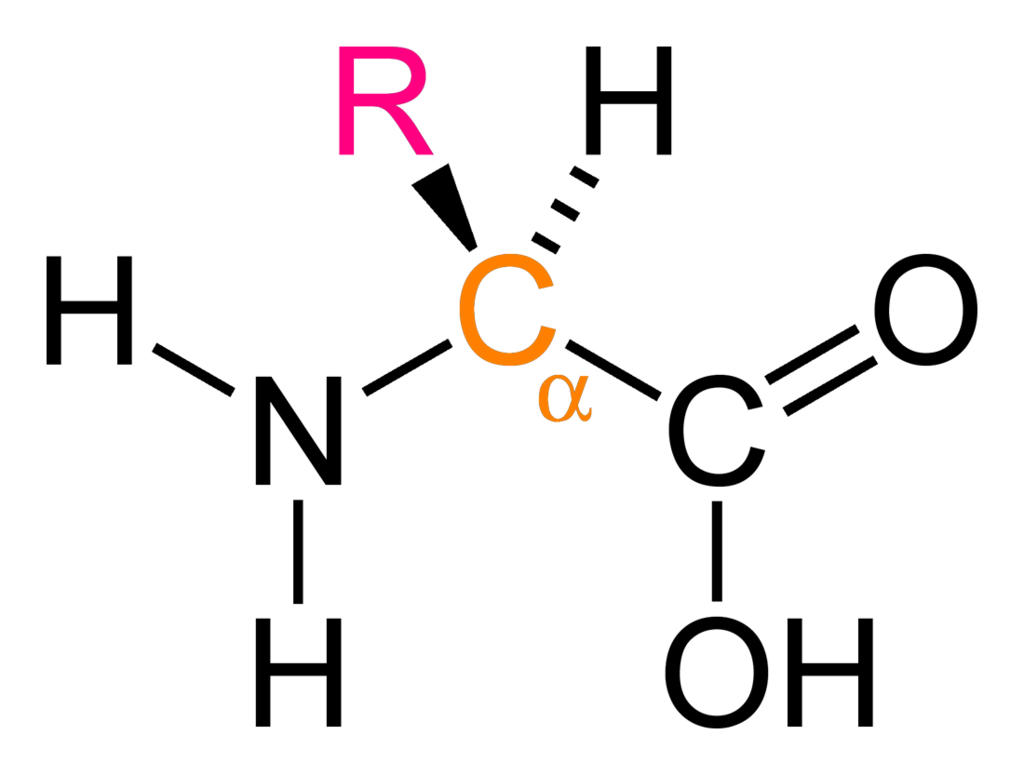
\includegraphics[height=4cm]{./figures/ch1/amino_acid_structure}
			\caption{La structure chimique d'un acide aminé.}
			\label{fig:amino_acid_structure}
		\end{subfigure}
		~
		\begin{subfigure}{.59\textwidth}
			\centering
			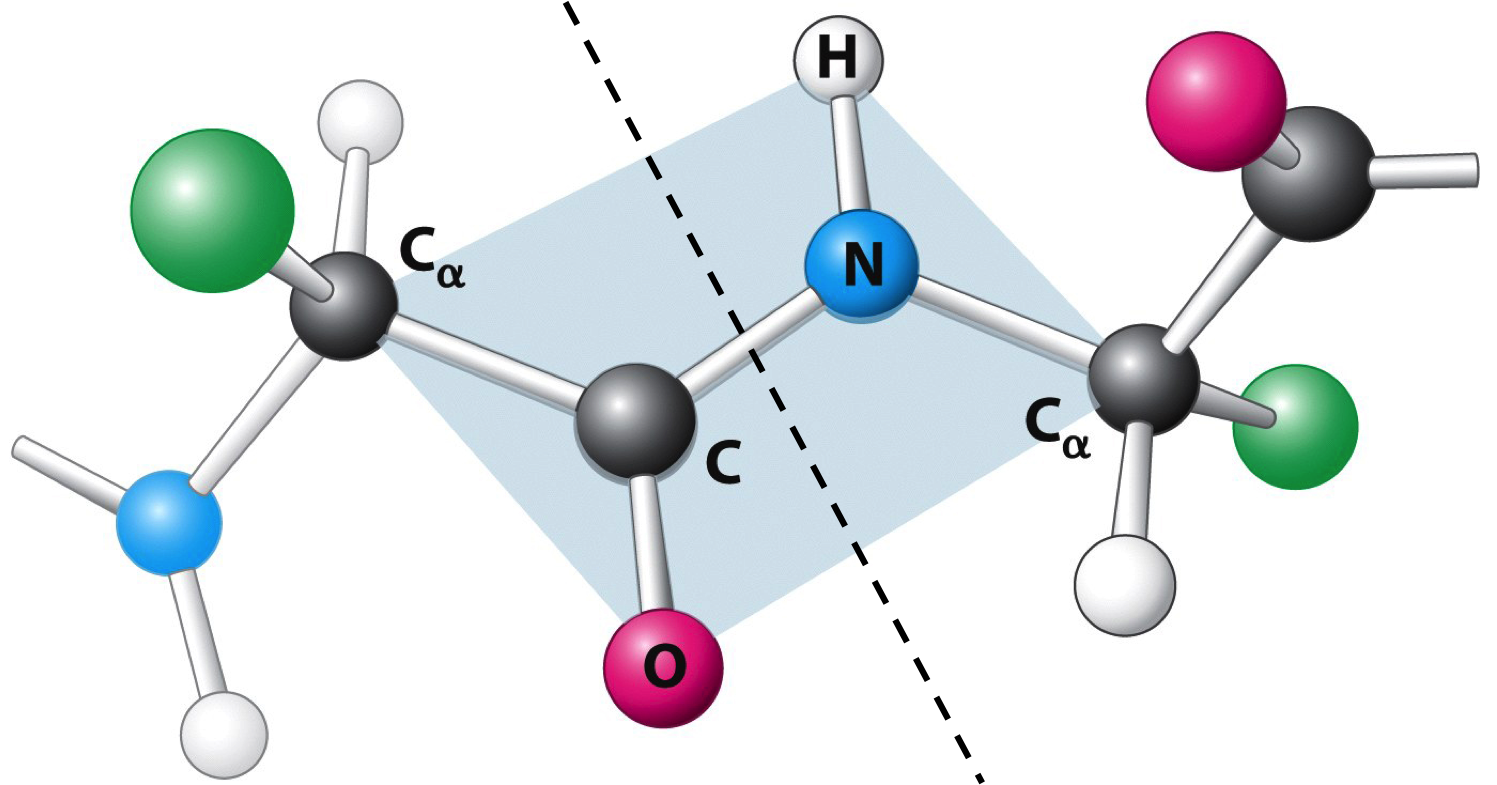
\includegraphics[height=4cm]{./figures/ch1/peptidic_bond.png}
			\caption{Illustration d'une liaison peptidique entre deux acides aminés (à gauche et à droite de la ligne pointillée). Cette liaison est une liaison covalente entre l'azote (N) de l'acide aminé de droite et le carbone (C) de l'acide aminé de gauche.}
			\label{fig:peptide_bond}
		\end{subfigure}
		\caption[Acide aminé]{Représentation schématique d'un acide aminé et d'une liaison petptidique. Crédit :~\cite{berg_biochemistry_2012}}
		\label{fig:aminoAcid}
	\end{figure}
	
	\begin{figure}[htb]
		\centering
		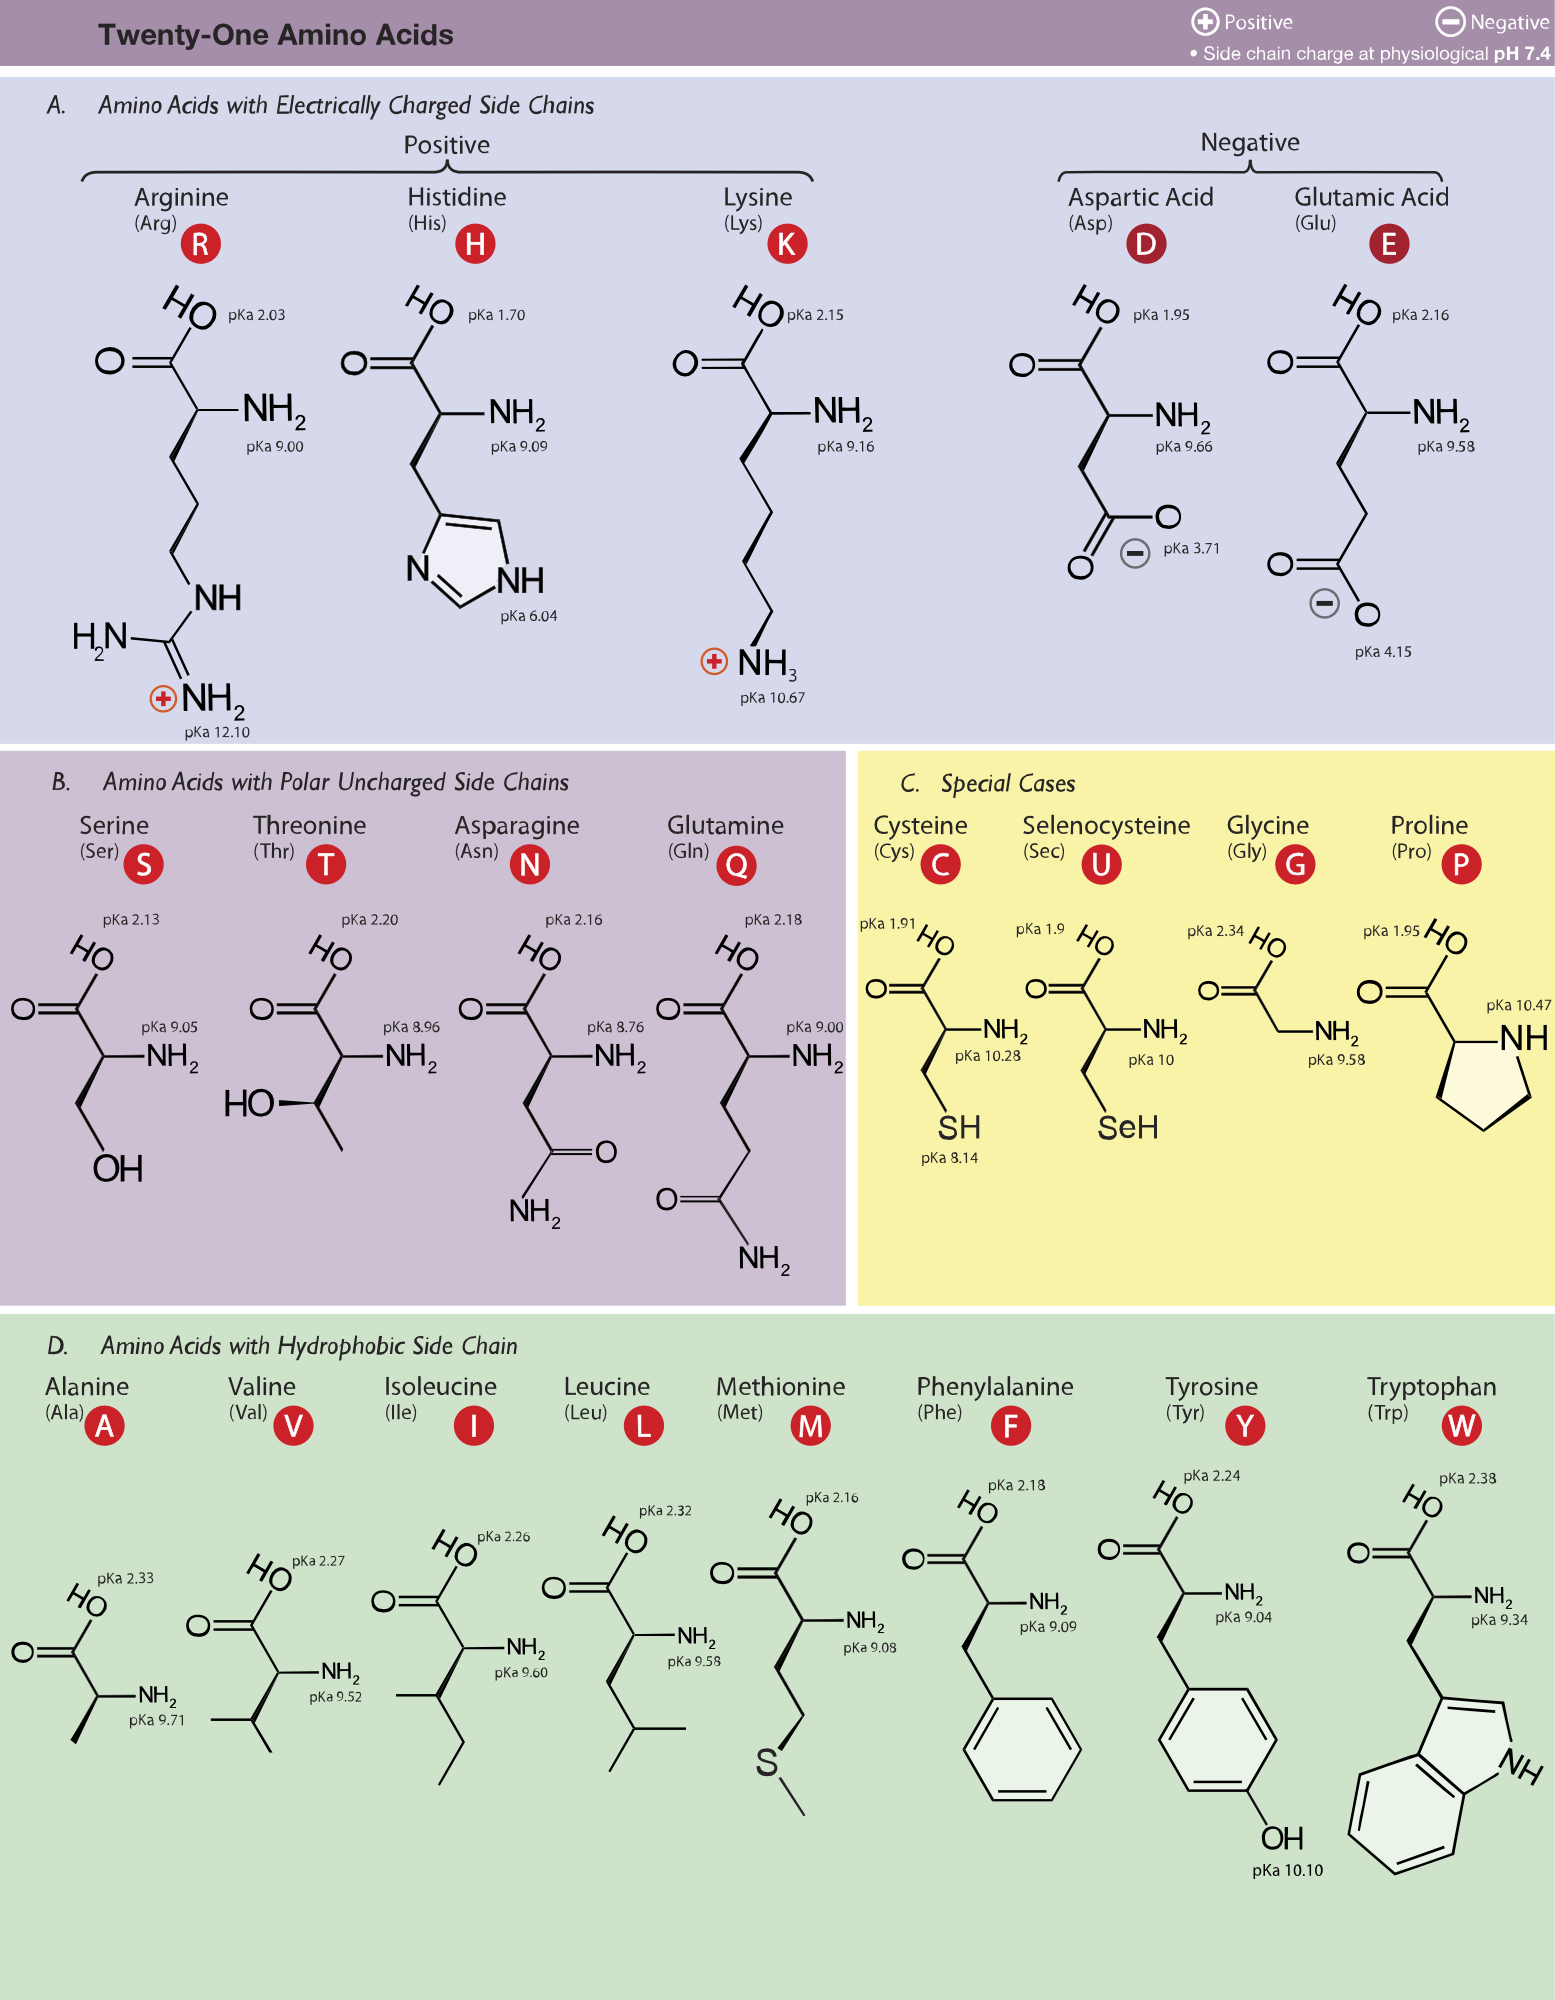
\includegraphics[width=0.9\textwidth]{figures/ch1/aminoAcids}
		\caption[Ensemble des acides aminés]{Les 21 acides aminés dits protéinogènes que l'on trouve chez les eucaryotes, c'est-à-dire ceux qui sont incorporés dans leurs protéines lors de la traduction de l'ARN messager par les ribosomes --- des complexes ribonucléoprotéiques dont la fonction est de synthétiser les protéines. Sur cette illustration, les acides aminés sont groupés en fonction des propriétés de leurs chaînes latérales, ici représentées \og au bas \fg{} des acides aminés. Crédit : \emph{Wikimedia}.}
		\label{fig:aminoAcids}
	\end{figure}
	
	\subsubsection{Synthèse}
	Un gène est un brin d'ADN qui \og code \fg{}  une protéine. Dans la cellule, ce brin d'ADN, composé de quatre nucléotides différents : adénine, cytosine, guanine et thymine (A, C, G, T) subit une \emph{transcription} en un brin d'ARN messager, composé également d'adénine, cytosine et guanine, mais d'uracil à la place de la thymine (A, C, G, U). Par exemple, la séquence \texttt{TAGTTCCAGTCAGT} serait transcrite en \texttt{UAGUUCCAGUCAGU}. Si l'ADN a pour fonction de stocker l'information génétique, l'ARN messager permet, comme son nom l'indique, de la communiquer au ribosome, un complexe moléculaire chargé de l'étape de \emph{traduction}.
	
	La traduction se fait selon le \emph{code génétique} illustré par la figure~\ref{fig:geneCode}. Ainsi, à chaque \emph{codon} (non-stop) est associé un acide aminé.
	
	\begin{figure}[htb]
		%\centering
		\begin{subfigure}[t]{0.44\textwidth}
			\centering
			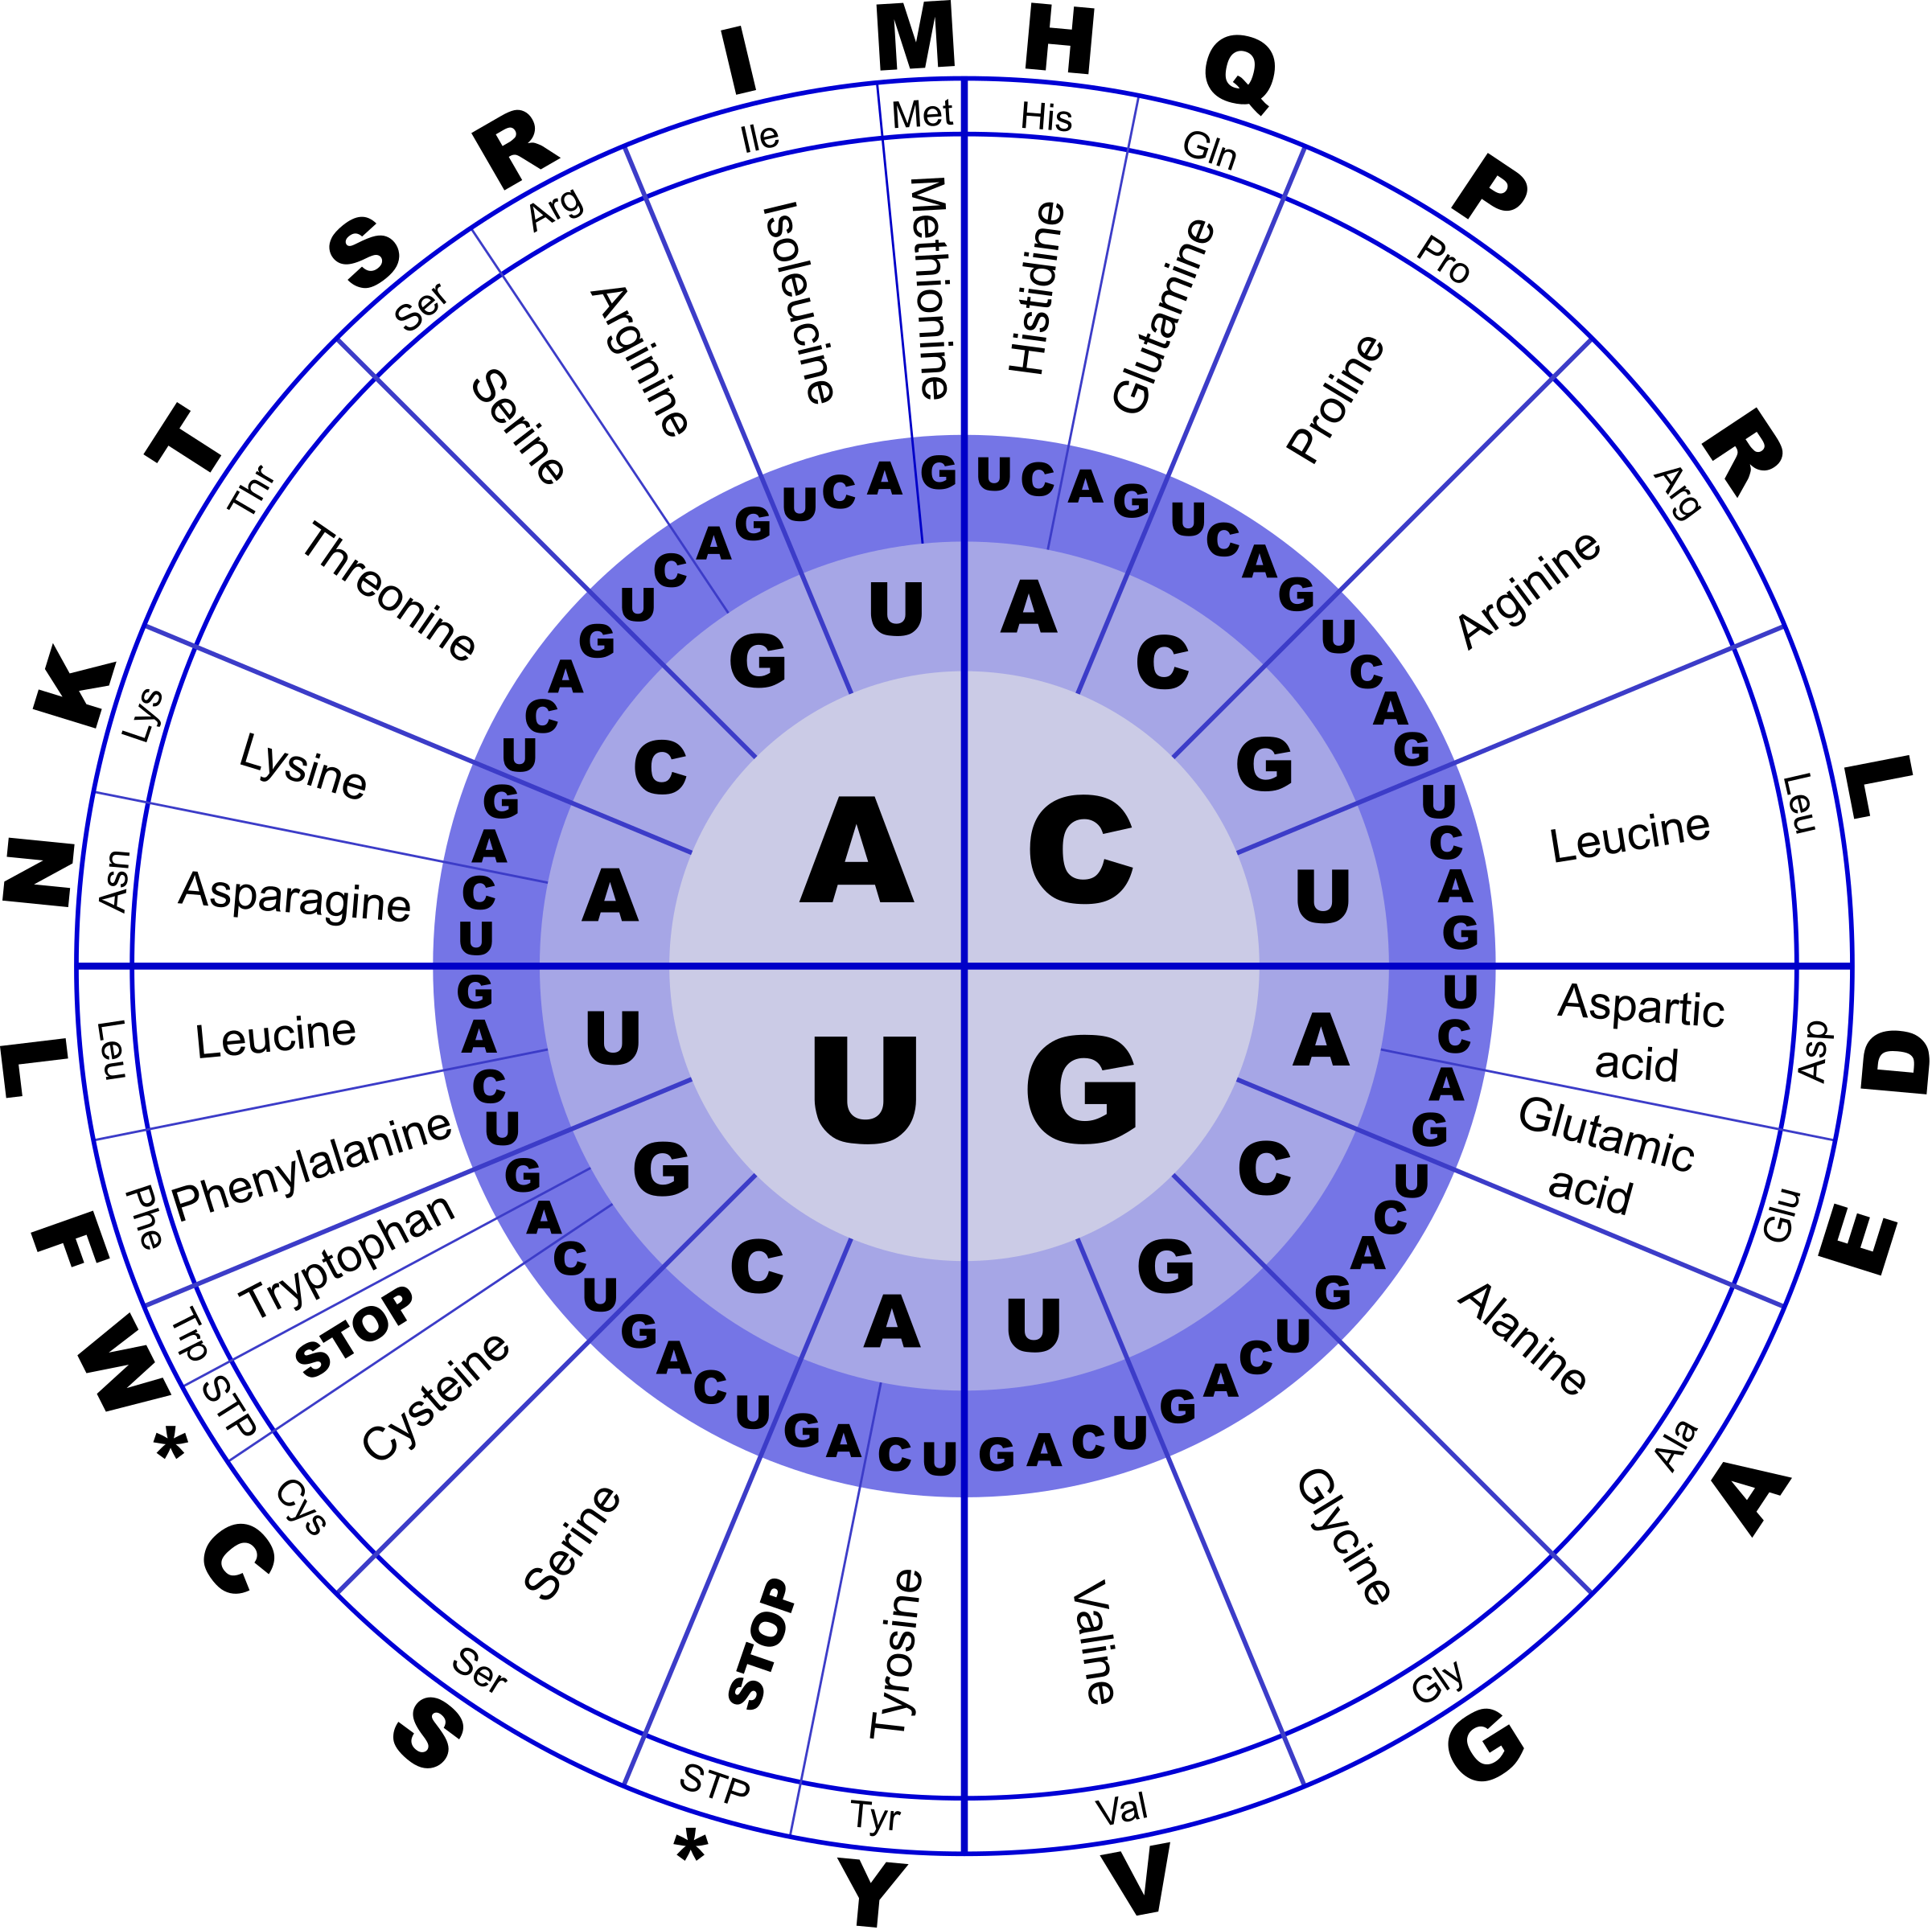
\includegraphics[width=\textwidth]{figures/ch1/geneCode}
			\caption[Le code génétique]{Ce diagramme illustre la correspondance entre un \emph{codon}, c'est-à-dire une suite de trois nucléotides (par exemple \texttt{UCG}) et l'acide aminé associé (dans le même exemple, la serine). On lit un codon du centre vers la périphérie du diagramme. Crédit : J\_{}Alves\footnotemark{}.}
			\label{fig:geneCode}
		\end{subfigure}
		~
		\begin{subfigure}[t]{0.54\textwidth}
			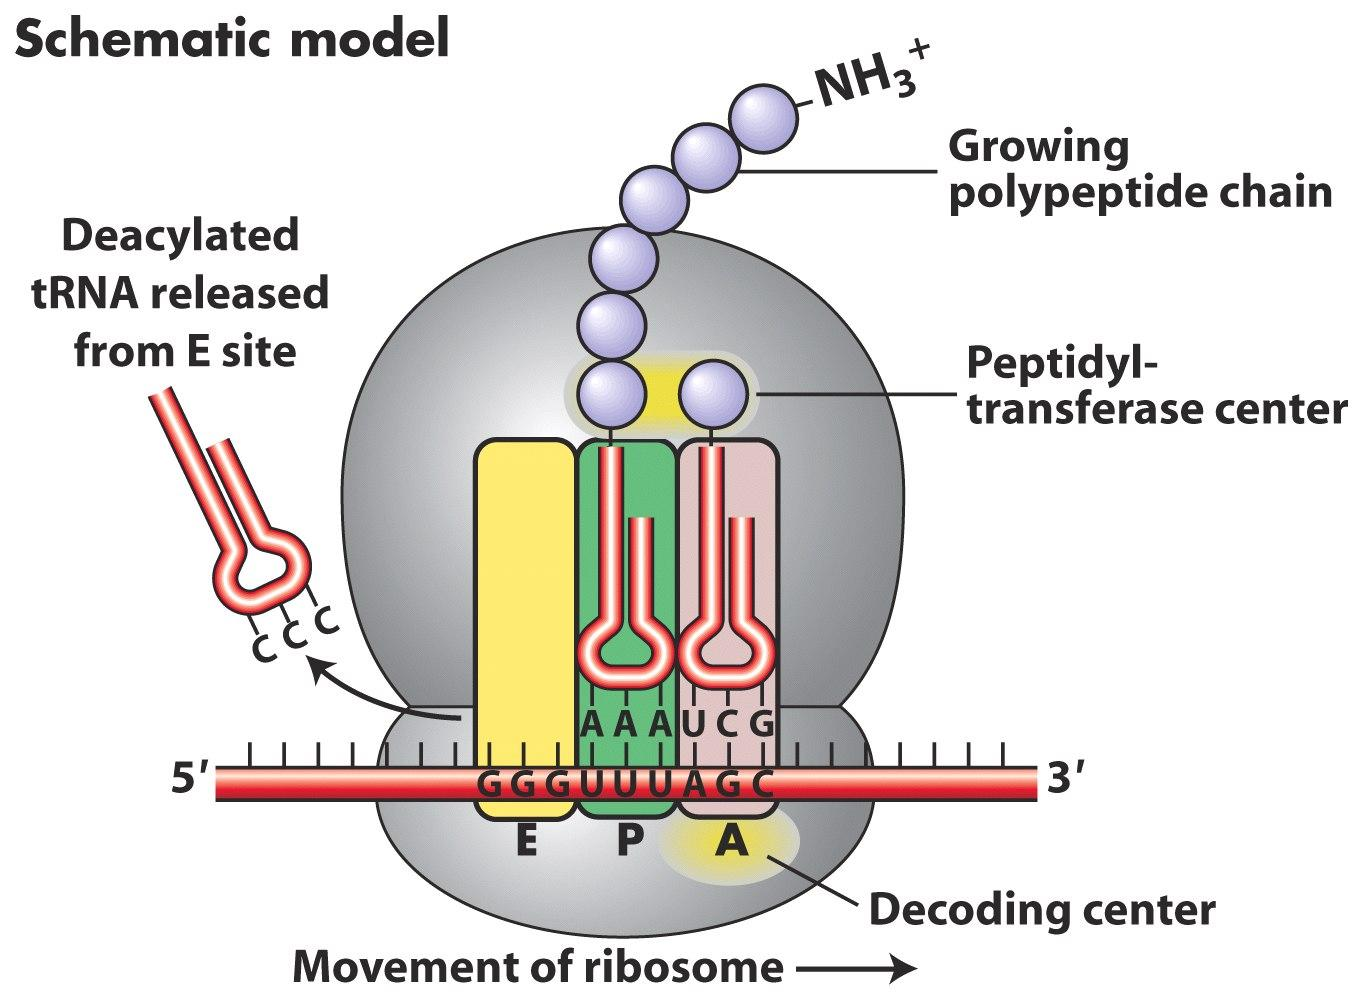
\includegraphics[width=\textwidth]{figures/ch1/translation}
			\caption[Traduction de l'ARN messager en protéine]{Traduction de l'ARN messager et synthèse d'une chaîne polypeptidique. Des ARN de transfert apportent les acides aminés au ribosome qui, en les liant aux bons codons sur le brin d'ARN messager, construit la chaîne polypeptidique dont la protéine finale sera constituée. Crédit : Liberty Voice\footnotemark{}.}
			\label{fig:translation}
		\end{subfigure}
		\label{fig:codeTrans}
		\caption{Code génétique et traduction.}
	\end{figure}
	
	\addtocounter{footnote}{-1}
	\footnotetext{\url{https://openclipart.org/detail/95203/genetic-code-rna}}
	\addtocounter{footnote}{1}
	\footnotetext{\url{http://guardianlv.com/2013/10/naked-mole-rat-longevity-explained-by-higher-translational-fidelity}}
	
	Le ribosome peut ainsi synthétiser une protéine à partir d'un brin d'ARN messager en associant le bon acide aminé à chaque codon, comme l'illustre le montre la figure
	
	\subsubsection{Structure}
	Les protéines sont décrites selon plusieurs niveaux de structures. On appelle structure primaire, la suite d'acides aminés qui composent la protéine, résultat de la traduction séquentielle d'un gène de l'ADN en protéine selon les règles du code génétique universel, dans lequel à chacun des 64 triplets possibles de nucléotides (A,C,G,T) composant l'ADN, correspond à un acide aminé. À ce niveau de structure, c'est la séquence qui est importante, la protéine étant considérée comme un collier de perles, chaque perle étant un des 22 acides aminées.
	
	Ensuite, pendant et après la synthèse, les protéines s'organisent en 3D pour former des architectures typiques, et cette organisation correspond à la structure secondaire~\cite{foltmann1981protein} qui est en fait une description de la structure tridimensionnelle localement adoptée par un segment de molécule. Cette structure secondaire s'explique par les liaisons hydrogène qui connectent et rapprochent spatialement certains segments, plus précisément entre les groupements amide et carbonyle du squelette peptidique, dans le cas des protéines, et entre les bases nucléiques dans le cas des acides nucléiques (acide désoxyribonucléique, ou ADN, et acide ribonucléique, ou ARN). Parfois, cette définition est assouplie et un segment peut être considéré comme une structure secondaire particulière sur la base des valeurs de certains de ses angles dièdres, indépendamment des liaisons hydrogène. Les algorithmes couramment utilisés pour identifier les structures secondaires incluent DSSP~\cite{kabsch1983dictionary}, \emph{Define}~\cite{richards1988identification}, \emph{Stride}~\cite{frishman1995knowledge} et SST~\cite{konagurthu2012minimum}.
		
	Dans la majorité des cas, une structure secondaire est soit une hélice alpha, soit un feuillet bêta~\cite{pauling1951structure}, soit un segment sans architecture ni contrainte appelé boucle. Dans une représentation dite \og en structures secondaires \fg{} ces segments de molécule sont remplacés par des représentations plus schématiques. Un exemple pour une hélice alpha est présenté dans la figure~\ref{fig:aHelix}, et un exemple pour un feuillet bêta est fourni sur la figure~\ref{fig:bSheet}. L'utilisation de ces schématisations permet de considérablement simplifier la représentation de la molécule finale, comme l'illustre la figure~\ref{fig:4awn_ss}.
	
	\begin{figure}[H]
		%\centering
		\begin{subfigure}[b]{.49\textwidth}
			\centering
			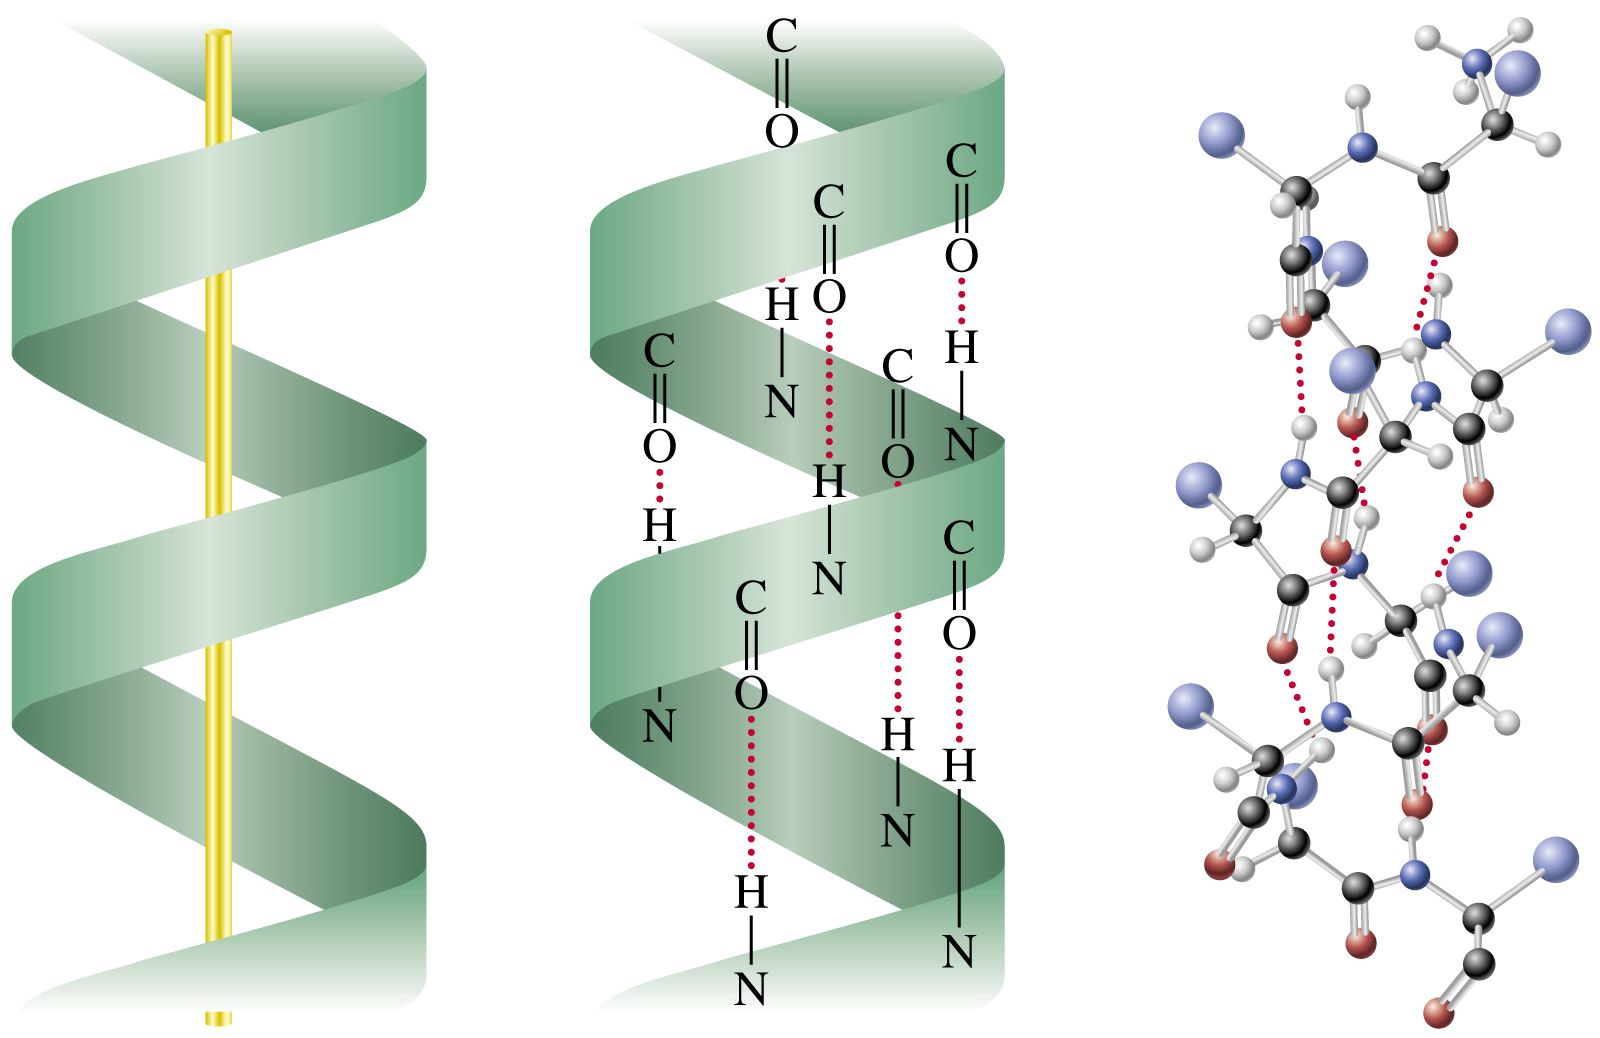
\includegraphics[width=\textwidth]{./figures/ch1/aHelix}
			\caption[Hélices alpha, trois représentations différentes]{Une hélice alpha schématisée (gauche), avec du texte représentant les atomes (centre) et en représentation \og tout atome \fg{} (droite). Lors d'un affichage \og en structures secondaires \fg{} la représentation de gauche est plus courante. Crédit : \emph{Bioinformatics -- An Introduction}, Bioinformatics Lab, AU\footnotemark.}
			\label{fig:aHelix}
		\end{subfigure}
		~
		\begin{subfigure}[b]{.49\textwidth}
			\centering
			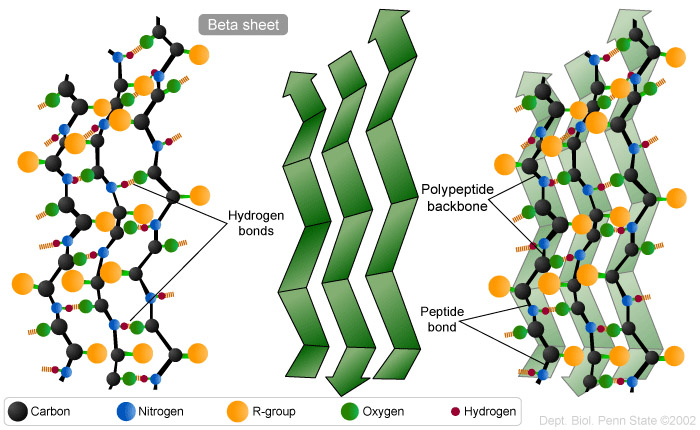
\includegraphics[width=\textwidth]{./figures/ch1/bSheet}
			\caption[Feuillets bêta]{Un feuillet bêta en représentation \og tout atome \fg{} (à gauche), sous forme schématique (au milieu), et en représentation \og tout atome \fg{} mixte (à droite). Lors d'un affichage \og en structures secondaires \fg{} la représentation du milieu est généralement choisie. Crédit : \emph{Department of Biology} -- PSU\footnotemark.}
			\label{fig:bSheet}
		\end{subfigure}
		\caption{Structures secondaires.}
		\label{fig:secStructs}
	\end{figure}
	
	\addtocounter{footnote}{-1}
	\footnotetext{\url{http://bioinfo.au-kbc.org.in/books/bi/1.html}}
	\addtocounter{footnote}{1}
	\footnotetext{\url{https://wikispaces.psu.edu/display/Biol230WCE/Properties+of+Macromolecules+I-Proteins}}
		
	De plus, ces représentations schématiques correspondent à des critères physiques ou chimiques précis et pertinents pour l'analyse des molécules concernées. La représentation en structures secondaires permet donc de simplifier la représentation tout en communicant efficacement des informations précises sur la molécule affichée~\cite{richardson2002teaching}. Le nombre d'objets différents (et de triangles, si des maillages sont utilisés) et très fortement réduit, ce qui améliore les performances d'affichage. Surtout, la molécule devient plus facile à observer, sa structure est plus lisible, et le niveau d'occultation des zones internes ou en arrière-plan de la molécule est considérablement diminué.
		
	Toutefois, l'utilisation de cette technique de visualisation implique une perte d'information. En effet, les atomes ne sont plus visibles, aussi la composition précise de la molécule n'est-elle plus perceptible. De fait, il devient difficile d'apprécier certaines propriétés du système, comme les champs électrostatiques, l'hydrophobicité, les cavités de la surface moléculaire et autres zones susceptibles de faciliter les interactions avec d'autres molécules. Il est cependant possible de représenter certaines de ces propriétés par des couleurs, par exemple.
		
	La représentation en structures secondaires est très courante, notamment pour visualiser des trajectoires\footnote{Dans le contexte de la dynamique moléculaire, on appelle \og trajectoire \fg{} l'évolution du système dans le temps, en particulier l'évolution des positions et des vélocités des particules simulées.} de dynamique moléculaire. Cette raison suffit à en faire une application majeure pour une technique de sélection de cibles mobiles. Le niveau d'occultation est particulièrement faible (relativement aux autres représentations, mais il reste élevé dans l'absolu) et les cibles, assez grosses, bougent relativement peu.
		
	Cependant, en pratique, il est courant d'associer à une représentation en structures secondaires la représentation \og tout atome \fg{} d'une partie de la molécule, généralement la partie que l'on soupçonne d'interagir avec une autre molécule, d'être un site d'arrimage, ou de présenter un autre intérêt particulier. Il en résulte une situation hybride, avec des cibles très mobiles et petites, mais un degré d'occultation global réduit. Cela permet de réduire le nombre de cibles potentielles, mais ce n'est possible qu'à condition de savoir \emph{a priori} qu'un sous-ensemble d'atomes --- et seulement ce sous-ensemble --- est susceptible d'être choisi par l'utilisateur, ce qui n'est pas toujours possible. La figure~\ref{fig:myoglobin} est un exemple de cette représentation hybride.

	Dans la littérature anglo-saxonne, la représentation en structures secondaires est parfois appelée \emph{cartoon} ou \emph{ribbons}~\cite{carson1986algorithm, richardson2000early}.
	
	\subsubsection{Rôles}
	Les protéines sont impliquées dans la plupart des processus biologiques et, de fait, leurs rôles sont extrêmement divers. On peut toutefois les diviser en deux grandes parties : les fonctions cellulaires et les fonctions biochimiques. Les premières définissent le rôle de la protéine dans la cellule ou l'organisme, et peuvent être découpées en cinq groupes~\cite{lodish1995molecular} :
	\begin{enumerate}
		\item Les protéines des structures, qui permettent à la cellule de maintenir son intégrité physique et son organisation dans l'espace. C'est par exemple la fonction du collagène, la protéine la plus abondante chez les mammifères~\cite{di2002mapping}.
		\item Les protéines de transport, qui acheminent les molécules nécessaires aux fonctions cellulaires au sein des cellules, mais aussi à travers les membranes nucléaires et plasmiques, ou hors des cellules. Cela inclut notamment le transport de dioxygène par l'hémoglobine, de fer par la transferrine~\cite{crichton1987iron} ou d'ions à travers les membranes cellulaires, par les canaux ioniques. 
		\item Les protéines régulatrices, qui inhibent ou stimulent l'activité d'autres protéines, ou la transcription de gènes, ce qui permet réguler divers processus biologiques.
		\item Les protéines de signalisation, qui reçoivent les signaux extérieurs (en se liant aux molécules qui les transmettent ou en réagissant à leur contact) et assurent leur transmission vers la cellule, ou vers une autre zone de l'organisme. Les protéines de signalisation permettent notamment de réagir aux hormones ; lorsque celles-ci sont hydrophiles (et donc incapables de traverser la membrane cellulaire, composée de lipides), les protéines réceptrices sont transmembranaires, leur extrémité extérieure permet la fixation de l'hormone, tandis que l'extrémité intérieure transmet le signal. C'est notamment le cas des récepteurs de l'insuline~\cite{gammeltoft1984insulin}. Lorsque les hormones sont lipophiles et peuvent traverser la membrane, la protéine réagit à la fixation de l'hormone par un changement conformationnel qui lui permettra de transmettre le signal. 
		\item Les protéines motrices, qui permettent aux cellules ou aux organismes de se mouvoir. On peut citer par exemple la myosine, essentielle à l'activité musculaire des vertébrés~\cite{pollard1973acanthamoeba}.
	\end{enumerate}	

	
	\FloatBarrier \subsection{Modes de représentation}
	Un atome n'est pas un objet au sens où on l'entend communément, dans un contexte macroscopique. S'il est courant de représenter un atome par une sphère, il n'a pas de rayon, de \og coquille \fg{} et ce n'est qu'une représentation schématique de la réalité, utilisée pour communiquer une information. Autour du noyau de l'atome se trouve un nuage électronique où les électrons occupent de manière probabiliste certaines régions de l'espace. Pour représenter ce nuage électronique, on peut procéder comme sur la figure~\ref{fig:helium}.

	
	\begin{wrapfigure}{O}{0.46\textwidth}
		\centering
		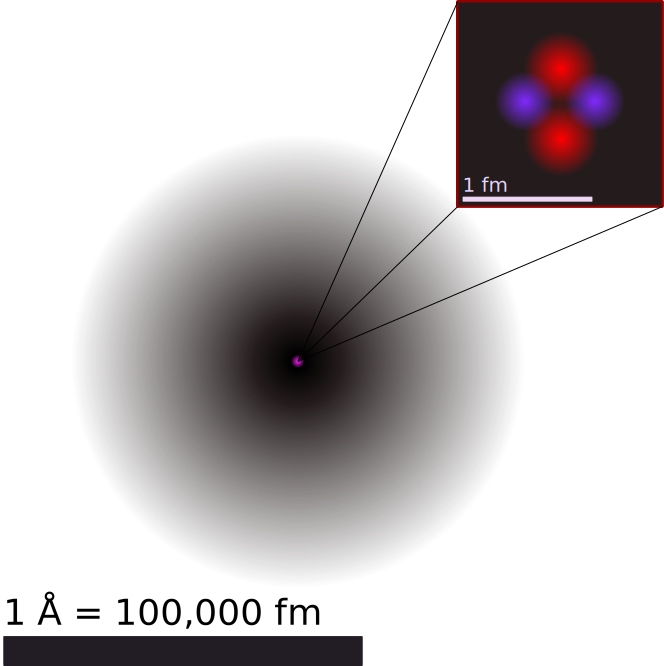
\includegraphics[width=0.44\textwidth]{figures/ch1/helium}
		\caption[Un atome d'hélium avec son nuage électronique]{Un atome d'hélium, avec le noyau en rose et la distribution du nuage électronique en nuances de gris. Le noyau de l'hélium-4 est représenté de façon très schématisée. La barre noire en bas indique l'échelle, et mesure $0,1$ nanomètre. Le dessin d'une \og coque \fg{}  pour représenter un atome sous forme de sphère de rayon fini est un choix arbitraire, dont l'importance pour la sélection d'atomes est déterminante. Crédit : \emph{Wikimedia}.}
		\label{fig:helium}
	\end{wrapfigure}
	
	\subsubsection{Points} Le mode de visualisation le plus simple consiste à représenter chaque atome (et uniquement les atomes) par un point tout juste assez gros pour être visible. Les liaisons covalentes ne sont pas représentées. Selon la façon dont elle est mise en œuvre, cette technique de visualisation peut être très performante, et donc garantir un affichage fluide même avec de très nombreux atomes. Elle a de plus l'avantage de minimiser l'occultation des atomes les uns par les autres, du fait de leur petite taille. Cependant, elle communique peu d'informations sur la molécule. En particulier, les liaisons covalentes étant absentes, sa structure même fait défaut. De plus, l'utilisateur peut difficilement se faire une idée de l'espace qu'occupe réellement cette molécule dans son milieu, car chaque atome n'est représenté que schématiquement, par un point bien plus petit que ce que l'on observe sur la figure~\ref{fig:helium}, par exemple.
		
	Enfin, elle rend difficile l'appréciation de la position d'un atome par rapport à ceux qui, dans le plan de l'écran (projeté) se trouvent à proximité, car seule la taille du point permet d'estimer sa distance par rapport à l'observateur. Or, comme les atomes ne font pas tous précisément la même taille, cette appréciation ne peut être que très approximative, même dans le cas où la couleur du point indiquerait la nature de l'atome représenté à un utilisateur connaissant la taille de l'atome en question. La figure~\ref{fig:4awn_points} présente un exemple de cette technique de visualisation. L'on comprend que, si la représentation en points présente certains avantages par rapport à une tâche de sélection, elle est par ailleurs trop limitée pour être appréciée des physico-chimistes ou biologistes souhaitant interagir avec des simulations moléculaires.
	    
	\subsubsection{Bâtons ou réglisse} Un autre mode de visualisation assez simple consiste à représenter uniquement les liaisons covalentes par des traits ou bâtons, juste assez épais pour être clairement visibles, ou par de petits cyclindes ou parallélépipèdes rectangles. Cette représentation est aussi parfois appelée \og réglisse \fg{} ou \emph{licorice}, en anglais. Si les atomes eux-mêmes ne sont pas explicitement représentés, ils se trouvent à l'intersection des liaisons covalentes où à leurs extrémités, et la coloration de ces liaisons indique la nature des atomes qu'elles relient.
		
	Dans une moindre mesure, cette technique de visualisation reprend les avantages de celle en points, puisque le niveau d'occultation, s'il est plus élevé, demeure assez faible. Le coût en ressources de calcul n'est pas nécessairement plus élevé que pour la représentation en points, ce qui permet également d'obtenir de très bonnes performances, même lorsque l'on affiche des systèmes très complexes. Un exemple est fourni dans la figure~\ref{fig:4awn_licorice}.
		
	La visualisation en réglisse, puisqu'elle affiche les liaisons covalentes, représente la structure de la molécule, et la représente même particulièrement clairement. Ses propriétés physico-chimiques peuvent donc être déduites de la représentation, du moins par un utilisateur expert. Par ailleurs, la distance d'un atome par rapport à la caméra est un peu plus facile à apprécier, car l'utilisateur dispose de plus de repères visuels (bien que ceux-ci puissent également occulter totalement l'atome, rendant sa localisation encore plus difficile). Elle partage cependant un inconvénient avec la visualisation en points, puisqu'elle communique à peu près aussi mal l'espace occupé par la protéine, en la réduisant visuellement à son \og squelette \fg{}. Selon les cas, cet inconvénient peut être plus ou moins gênant.
		
	Cette représentation dispose de suffisamment d'avantages pour être utilisée assez fréquemment. Par conséquent, elle constitue un cas d'application important pour les contributions présentées plus loin.
		
	\subsubsection{Boules et bâtons, ou CPK} Une technique de visualisation très courante est appelée \og en boules et bâtons \fg{} (ou \emph{ball-and-stick}, en anglais). Elle est parfois appelée CPK, un peu par abus de langage, en référence aux modèles physiques créés par les chimistes Robert \textbf{C}orey, Linus \textbf{P}auling, et améliorés par Walter \textbf{K}oltun~\cite{corey1953molecular, koltun1965space} ainsi qu'à la convention de couleurs CPK qui est souvent utilisée avec cette représentation. Cette convention est essentiellement caractérisée par l'utilisation du noir pour le carbone, du blanc pour l'hydrogène, du rouge pour l'oxygène, du bleu pour l'azote, du jaune pour le soufre, du violet pour le phosphore, de nuances de vert pour les halogènes (fluore, chlore, brome, iode) et du gris argent pour les métaux.
		
	Ce mode de visualisation, que nous désignerons ci-après par l'appellation \emph{CPK}, représente chaque atome par une sphère, et chaque liaison covalente par un bâton, comme dans la représentation par bâtons. Il s'agit comme dans cette dernière de bien représenter la structure de la molécule, mais en insistant plus sur les atomes. Traditionnellement, ceux-ci sont toutefois représentés par des sphères nettement plus petites que le rayon de van der Waals des atomes (voir le mode suivant).
		
	Outre le fait qu'elle correspond aux modèles physiques CPK, comme celui de la figure~\ref{fig:aspirin}, cette représentation permet de bien visualiser la structure de la molécule et la nature de ses atomes. Naturellement, l'utilisation de sphères implique un degré d'occultation accru par rapport à la représentation en bâtons, mais elle permet aussi d'avoir une meilleure appréciation du volume occupé par la molécule.
		
	Sur ce dernier point, la représentation en boules et bâtons a néanmoins ses limites, puisqu'elle occupe un volume réduit par rapport à certaines références pertinentes d'un point de vue physico-chimique, liées au rayon de van der Waals ou à la densité moléculaire, comme détaillé dans les descriptions des représentations suivantes.
		
	\subsubsection{Sphères de van der Waals} La représentation en sphères de van der Waals (ou vdW) repose sur la notion de rayon de van der Waals. Celle-ci découle elle même de la force de van der Waals~\cite{dzyaloshinskii1961general}. Il s'agit en fait de l'effet combiné de plusieurs forces :
	
	\begin{itemize}
	    \item Les interactions électrostatiques (attractives et répulsives) entre des multipôles permanents, parfois appelées Forces de Keesom~\cite{keesom1915second} ;
		\item L'induction (ou polarisation), c'est-à-dire l'interaction électrostatique attractive entre un multipôle permanent et un multipôle induit, également appelée force de Debye~\cite{debye1913reprinted, debye1929polar} ;
	    \item La dispersion, c'est-à-dire l'interaction électrostatique attractive entre deux multipôles induits, aussi désignée force de London~\cite{eisenschitz1930verhaltnis, london1930theorie, london1937general} ;
		\item La répulsion de Pauli, qui découle du principe d'exclusion de Pauli~\cite{pauli1925zusammenhang}, selon lequel plusieurs électrons (et autres fermions) ne peuvent pas se trouver simultanément dans le même état quantique. En effet, attendu que les électrons de deux atomes ne peuvent pas occuper le même espace simultanément, des atomes dont les nuages électroniques se croisent sont soumis à une force répulsive.
	\end{itemize}
	
	Les logiciels de simulation utilisent fréquemment le potentiel de Lennard-Jones~\cite{lennard1924determination} pour modéliser les forces de van der Waals. Celui-ci peut s'exprimer par $E_{p}\left(r\right) = 4E_{0} \left( \left(\frac{d}{r}\right)^{12} - \left(\frac{d}{r}\right)^{6} \right)$, où $r$ est la distance entre les centres des deux atomes concernés, et $d$ représente la distance pour laquelle le potentiel de Lennard-Jones est nul ; $E_{0}$ est la valeur minimale du potentiel, soit le \og fond \fg{} du puits de potentiel. Comme on l'observe aisément sur la figure~\ref{fig:lennard}, le potentiel admet un minimum, dont on peut déduire un rayon de van der Waals. Ce rayon peut être celui d'une sphère représentant l'atome en question.
 
	C'est le principe de la représentation en sphères de van der Waals, illustrée par la figure~\ref{fig:4awn_VdW}. Ce mode de visualisation a plusieurs avantages. Premièrement, il correspond à une réalité physique, celle des forces de van der Waals. Deuxièmement, il permet d'apprécier le volume occupé par la molécule. Troisièmement, les atomes étant représentés par de grosses sphères, ils sont mieux visibles pour un niveau de zoom donné. De fait, il est plus aisé d'envisager les interactions possibles entre cette molécule et une autre, puisque l'on perçoit mieux les volumes des cavités dans lesquelles d'éventuels ligands\footnotemark{} pourraient venir se loger, et la bonne visualisation des atomes à la surface peut aider à évaluer la probabilité d'un arrimage avec ledit ligand.
	
	\footnotetext{En biologie, un ligand est une molécule qui se lie de manière réversible sur une macromolécule ciblée, protéine ou acide nucléique, jouant en général un rôle fonctionnel : stabilisation structurale, catalyse, modulation d'une activité enzymatique, transmission d'un signal. Par exemple, le hème de la myoglobine est un ligand, cf. la figure~\ref{fig:myoglobin}.}
		
	Cependant, les liaisons covalentes sont totalement occultées, et il est seulement possible de les \og deviner \fg{} à partir de l'emplacement des atomes et grâce aux lois de la chimie. La structure de la molécule est donc beaucoup moins claire qu'en représentation CPK, par exemple. De plus, les atomes sont si gros qu'ils occultent totalement ceux qui sont derrière eux. De fait, l'intérieur de la molécule devient totalement invisible. Si sa surface est mieux représentée, sa structure interne est entièrement occultée. C'est plus gênant encore lorsque les atomes d'hydrogène sont affichés, ce qui n'est pas le cas sur la figure~\ref{fig:4awn_VdW} --- il est courant de les omettre, par souci de clarté. Selon la mise en \oe{}uvre logicielle de cette représentation, elle peut être coûteuse en ressources de calcul, même si des solutions efficaces existent. En mouvement, la grande taille des atomes a l'avantage de diminuer leur mouvement relatif, c'est-à-dire leur mouvement par rapport à eux-mêmes.
		
	Les sphères de van der Waals ne sont pas une mauvaise option pour visualiser (ou interagir avec) une simulation de dynamique moléculaire, à condition que l'objet d'intérêt principal soit superficiel, et donc bien visible. La grande taille des cibles peut être un avantage, même s'il y a un certain degré d'interpénétration entre elles. Cette représentation constitue donc un cas d'application notable pour une technique de sélection de cibles mobiles.
	
 	\begin{wrapfigure}{O}{0.45\textwidth}
 		\centering
 		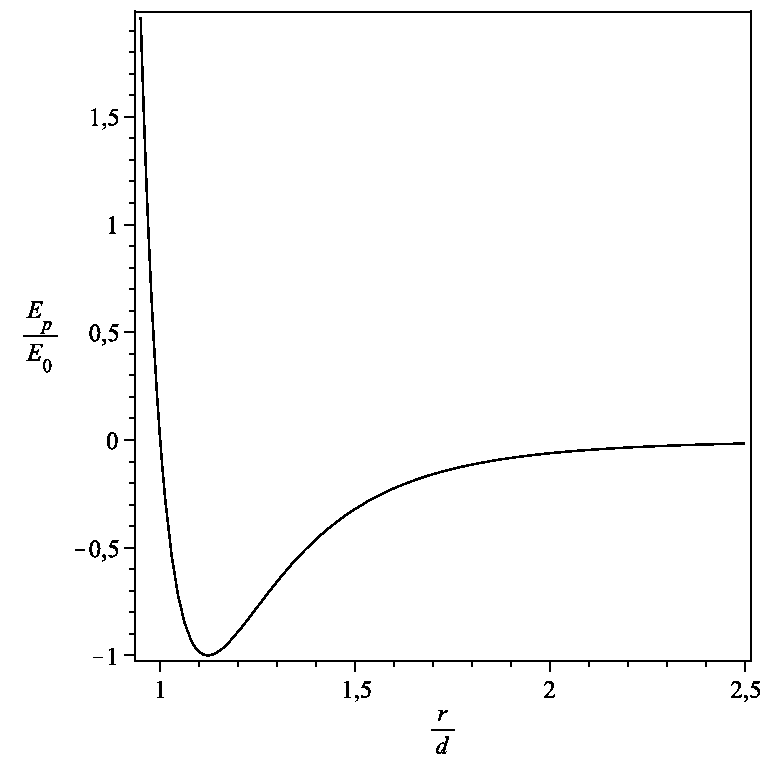
\includegraphics[width=0.41\textwidth]{figures/ch1/lennard-jones}
		\caption[Représentation graphique du potentiel de Lennard-Jones]{Représentation graphique du potentiel de Lennard-Jones, en fonction du rapport $r/d$ entre la distance interatomique réelle et celle pour laquelle le potentiel s'annule. Le potentiel admet un minimum en $r/d = 2^{1/6}$, soit environ $1,12$ ; ce minimum correspond au rayon de van der Waals. Crédit : \emph{Wikimedia}.}
 		\label{fig:lennard}
 	\end{wrapfigure}
	
	\subsubsection{\emph{Hyperballs}} La technique de visualisation de molécules appelée \emph{Hyperballs}~\cite{chavent2011gpu} se fonde sur une représentation analytique des atomes et des liaisons covalentes. Leurs surfaces sont décrites par des équations, des rayons sont lancés vers les atomes, et il s'agit ensuite de résoudre des équations d'intersection entre les rayons et les surfaces.
		
	Les \emph{Hyperballs} présentent de nombreux avantages. Sur le plan purement technique, leur mode de représentation analytique permet, au contraire des maillages de points (\emph{meshes}, en anglais), d'éviter d'avoir à gérer un très grand nombre de points et de triangles. De plus, quel que soit le niveau de zoom, les surfaces des sphères et des liaisons covalentes (représentées par des hyperboloïdes) demeurent parfaitement lisses.	Avec des maillages, il est nécessaire d'avoir un grand nombre de triangles pour maintenir l'illusion de la rotondité du modèle lorsqu'il est observé de près.
	
	En réalité, les illustrations fournies jusqu'ici pour la représentation en points, en bâtons, en boules et bâtons, et en sphères de van der Waals ont toutes été produites avec des \emph{Hyperballs}, simplement en jouant sur leurs paramètres. Cette grande flexibilité rend cette technique particulièrement avantageuse, surtout compte tenu des performances de premier ordre qu'elle offre~\cite{chavent2011gpu}.
		
	Au-delà de sa flexibilité, cependant, elle a l'avantage de permettre une représentation originale, avec des liaisons représentées par des hyperboloïdes. En jouant sur la courbure de ces hyperboloïdes, on peut communiquer des informations sur la nature de la liaison, par exemple sur la quantité d'énergie nécessaire à sa rupture. Si cette quantité est faible, on peut représenter la liaison par une hyperboloïde très \og creusée \fg{}, donnant l'impression d'être sur le point de rompre.
		
	Enfin, les \emph{Hyperballs}, utilisées de la façon la plus \og classique \fg{} ou \og canonique \fg{} présentent des hyperboloïdes partiellement creusées, comme sur la figure~\ref{fig:4awn_HB}. Cette représentation est souvent appréciée pour ses qualités esthétiques, certes subjectives. D'un point de vue plus objectif, la représentation en \emph{Hyperballs} canoniques présentent à peu près les mêmes caractéristiques que la représentation en boules et bâtons. Les dimensions sont proches, même si les formes diffèrent. Les liaisons sont un peu plus épaisses près des atomes, et comparables, voire un peu plus fines au milieu. De fait, la perception de la structure de la molécule et de ses propriétés, ainsi que le niveau d'occultation visuelle, sont assez comparables. Par conséquent, la représentation en \emph{Hyperballs} canoniques est un cas d'application aussi pertinent pour la sélection de cibles mobiles que la représentation CPK, voire plus, car les bonnes performances des \emph{Hyperballs} permettent de gérer de très gros systèmes plus facilement.
	
	\subsubsection{Surface accessible au solvant et surface de Connolly}
	Plutôt que de représenter les atomes d'une molécule, ou ses liaisons covalentes, ou sa structure interne de façon schématique, il est possible de représenter sa \og surface \fg{}. Attendu qu'une molécule n'est pas un objet macroscopique, le concept de surface est nécessairement plus abstrait, et il convient donc de préciser de quoi il s'agit. On peut en effet définir la surface moléculaire de plusieurs façons.
		
	Un définition très courante est la surface de Connolly~\cite{connolly1983analytical}, parfois également appelée \emph{solvent excluded surface} dans la littérature anglo-saxonne. Il s'agit de l'ensemble des points auxquels la molécule et \og le solvant \fg{} (généralement une sphère représentant une molécule d'eau) peuvent entrer en contact, où le contact est défini par le rayon de van der Waals.
	
	\begin{wrapfigure}{O}{0.42\textwidth}
		\centering
		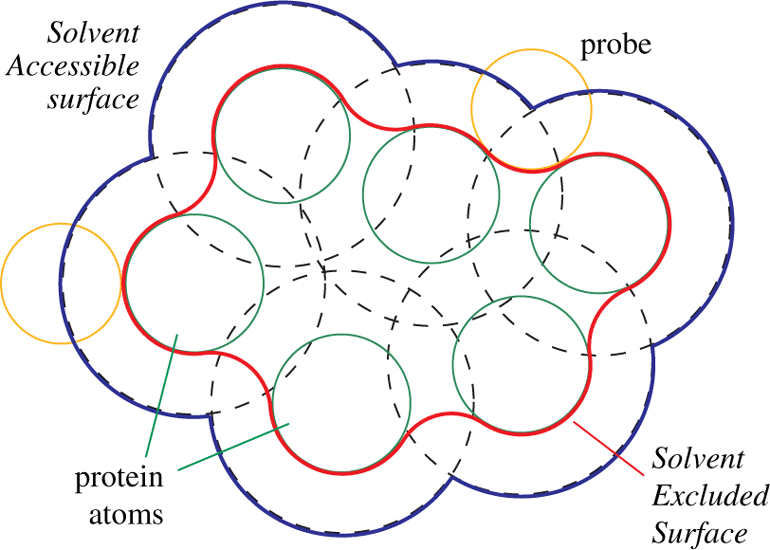
\includegraphics[width=0.40\textwidth]{figures/ch1/connolly}
		\caption[Surface de Connolly et accessible au solvant]{Surface de Connolly. Une sonde (cercles jaunes) est \og roulée \fg{} sur les atomes (verts) de la molécule, et son tracé est conservé en rouge : c'est la surface de Connolly. La surface tracée par le centre de la sonde est dite accessible au solvant. Cet algorithme est aussi appelé \emph{rolling ball}~\cite{shrake1973environment, connolly1983analytical, connolly1993molecular}. Crédit :~\cite{krone2009interactive}.}
		\label{fig:connolly}
	\end{wrapfigure}
	
	La figure~\ref{fig:connolly} illustre plus clairement ce principe. Une autre surface très courante est la surface accessible au solvant~\cite{lee1971interpretation}, définie par l'ensemble des points parcourus par le centre de la sphère représentant le solvant quand elle est en contact avec la molécule. C'est également illustré par la figure~\ref{fig:connolly}. Enfin, la figure~\ref{fig:4awn_ses} montre une protéine entière représentée par sa surface de Connolly.
		
	\subsubsection{Isosurface de densité} On peut également représenter une molécule par sa surface en se fondant sur un seuil de densité moléculaire. On calcule, dans une grille tridimensionnelle d'une résolution arbitraire, la densité en chaque case --- on construit un champ scalaire. Ensuite, on choisit arbitrairement un seuil de densité, et l'on trace une isosurface de densité à partir de ce seuil. On utilise généralement pour ce faire l'algorithme des \emph{marching cubes}~\cite{lorensen1987marching}.	L'isosurface de densité $D$ correspond à l'ensemble des points de l'espace dont la densité moléculaire vaut $D$.
	
	Outre le fait qu'elle représente une grandeur physique concrète, l'isosurface de densité a l'avantage d'être relativement rapide à calculer. En effet, l'algorithme \emph{QuickSurf}~\cite{krone2012fast, roberts2013lattice, stone2013early, stone2013gpu, stone2014gpu, sener2014visualization}, par exemple, permet de calculer une isosurface de densité suffisamment vite pour la recalculer en temps réel lors d'une simulation de dynamique moléculaire. Cet algorithme est conçu pour être exécuté sur un GPU (un processeur graphique, particulièrement adapté aux calculs très parallèles) ce qui améliore ses performances d'un à deux ordres de grandeur. Il permet de plus d'ajuster plusieurs paramètres : la résolution spatiale générale, le rayon des atomes (utilisé pour générer la grille de densité, par somme de gaussiennes 3D), l'isovaleur de densité voulue, la résolution de la grille de densité, et la distance de coupure utilisée pour la gaussienne associée à chaque atome\footnote{\url{http://www.ks.uiuc.edu/Research/vmd/current/ug/node73.html}}.
	
	Du fait des performances de cet algorithme et de sa souplesse, les isosurfaces de densité représentent un cas d'application intéressant. En effet, elles sont assez couramment utilisées en simulation de dynamique moléculaire, et présentent des caractéristiques très distinctes des modèles de représentation atomiques. Contrairement à ces derniers, elles ne présentent pas de (dizaines ou centaines) de milliers de cibles distinctes, mais un seul objet continu. De fait, au premier abord elles ne semblent pas nécessiter d'assistance à la sélection. Cependant, les nombreuses aspérités d'une isosurface, attendu qu'elles correspondent à celles de la molécule, peuvent être considérées comme des cibles distinctes, à condition d'avoir une méthode pour les distinguer. Cette méthode pourrait éventuellement être fondée sur des critères de concavité et convexité. Si l'on considère chaque sous-ensemble convexe d'une surface de densité avec un seuil élevé, par exemple, on aboutit à plusieurs dizaines de cibles potentielles ; et ce pour une protéine de taille relativement réduite (par exemple 2000 atomes, quand certaines protéines en comptent des dizaines de milliers). On peut également considérer les sous-ensembles concaves comme des cibles, car ils peuvent représenter des cavités ou tunnels\footnotemark{} dignes d'intérêt.
	
	\footnotetext{Les cavités et tunnels des protéines sont critiques pour la compréhension de phénomènes tels que la liaison de ligands, le transport moléculaire ou la catalyse enzymatique~\cite{paramo2014}.}
	
	On constate donc qu'une isosurface de densité peut présenter de nombreuses cibles mobiles, avec toutefois un niveau d'occultation réduit, puisque l'intérieur de la molécule n'est pas représenté. Les aspérités situées à \og l'arrière \fg{} de la molécule sont cependant totalement occultées. De plus, la représentation en isosurface est particulièrement prisée pour l'arrimage\footnote{\emph{docking}, en anglais} de protéines, qui implique au moins deux molécules et parfois beaucoup plus. Avec de nombreuses molécules, le nombre de cibles potentielles peut donc devenir très élevé, de même que la quantité de mouvement, puisqu'il faut ajouter au mouvement d'une aspérité d'une surface par rapport à elle-même le mouvement de toute la surface par rapport à l'environnement.
	
	\subsubsection{Autres techniques de représentation}
	La liste des techniques de représentation fournie ci-dessus ne saurait être considérée comme exhaustive. En effet, les logiciels de visualisation moléculaires sont nombreux, et les possibilités qu'ils offrent le sont encore plus. Des programmes couramment utilisés, tels que \emph{UnityMol}~\cite{doutreligne2014unitymol}, VMD~\cite{humphrey1996vmd}, \emph{PyMol}~\cite{delano2002pymol}, \emph{QuteMol}~\cite{tarini2006ambient, tarini2006qutemol}, \emph{Chimera(X)}~\cite{pettersen2004ucsf, goddard2017ucsf}, ~\emph{Yasara}~\cite{krieger2014yasara}, \emph{LigandScout}~\cite{wolber2005ligandscout} ou \emph{Jmol}~\cite{herraez2006biomolecules} proposent des options très diverses. En outre, les divers modes de représentation proposés par ces outils peuvent être combinés librement, comme sur la figure~\ref{fig:transSS}.
	
	
	\newcommand{\subImgW}{0.32\textwidth}
	\begin{figure}[!htbp]
		%\centering
		\begin{subfigure}[t]{\subImgW}
			\centering
			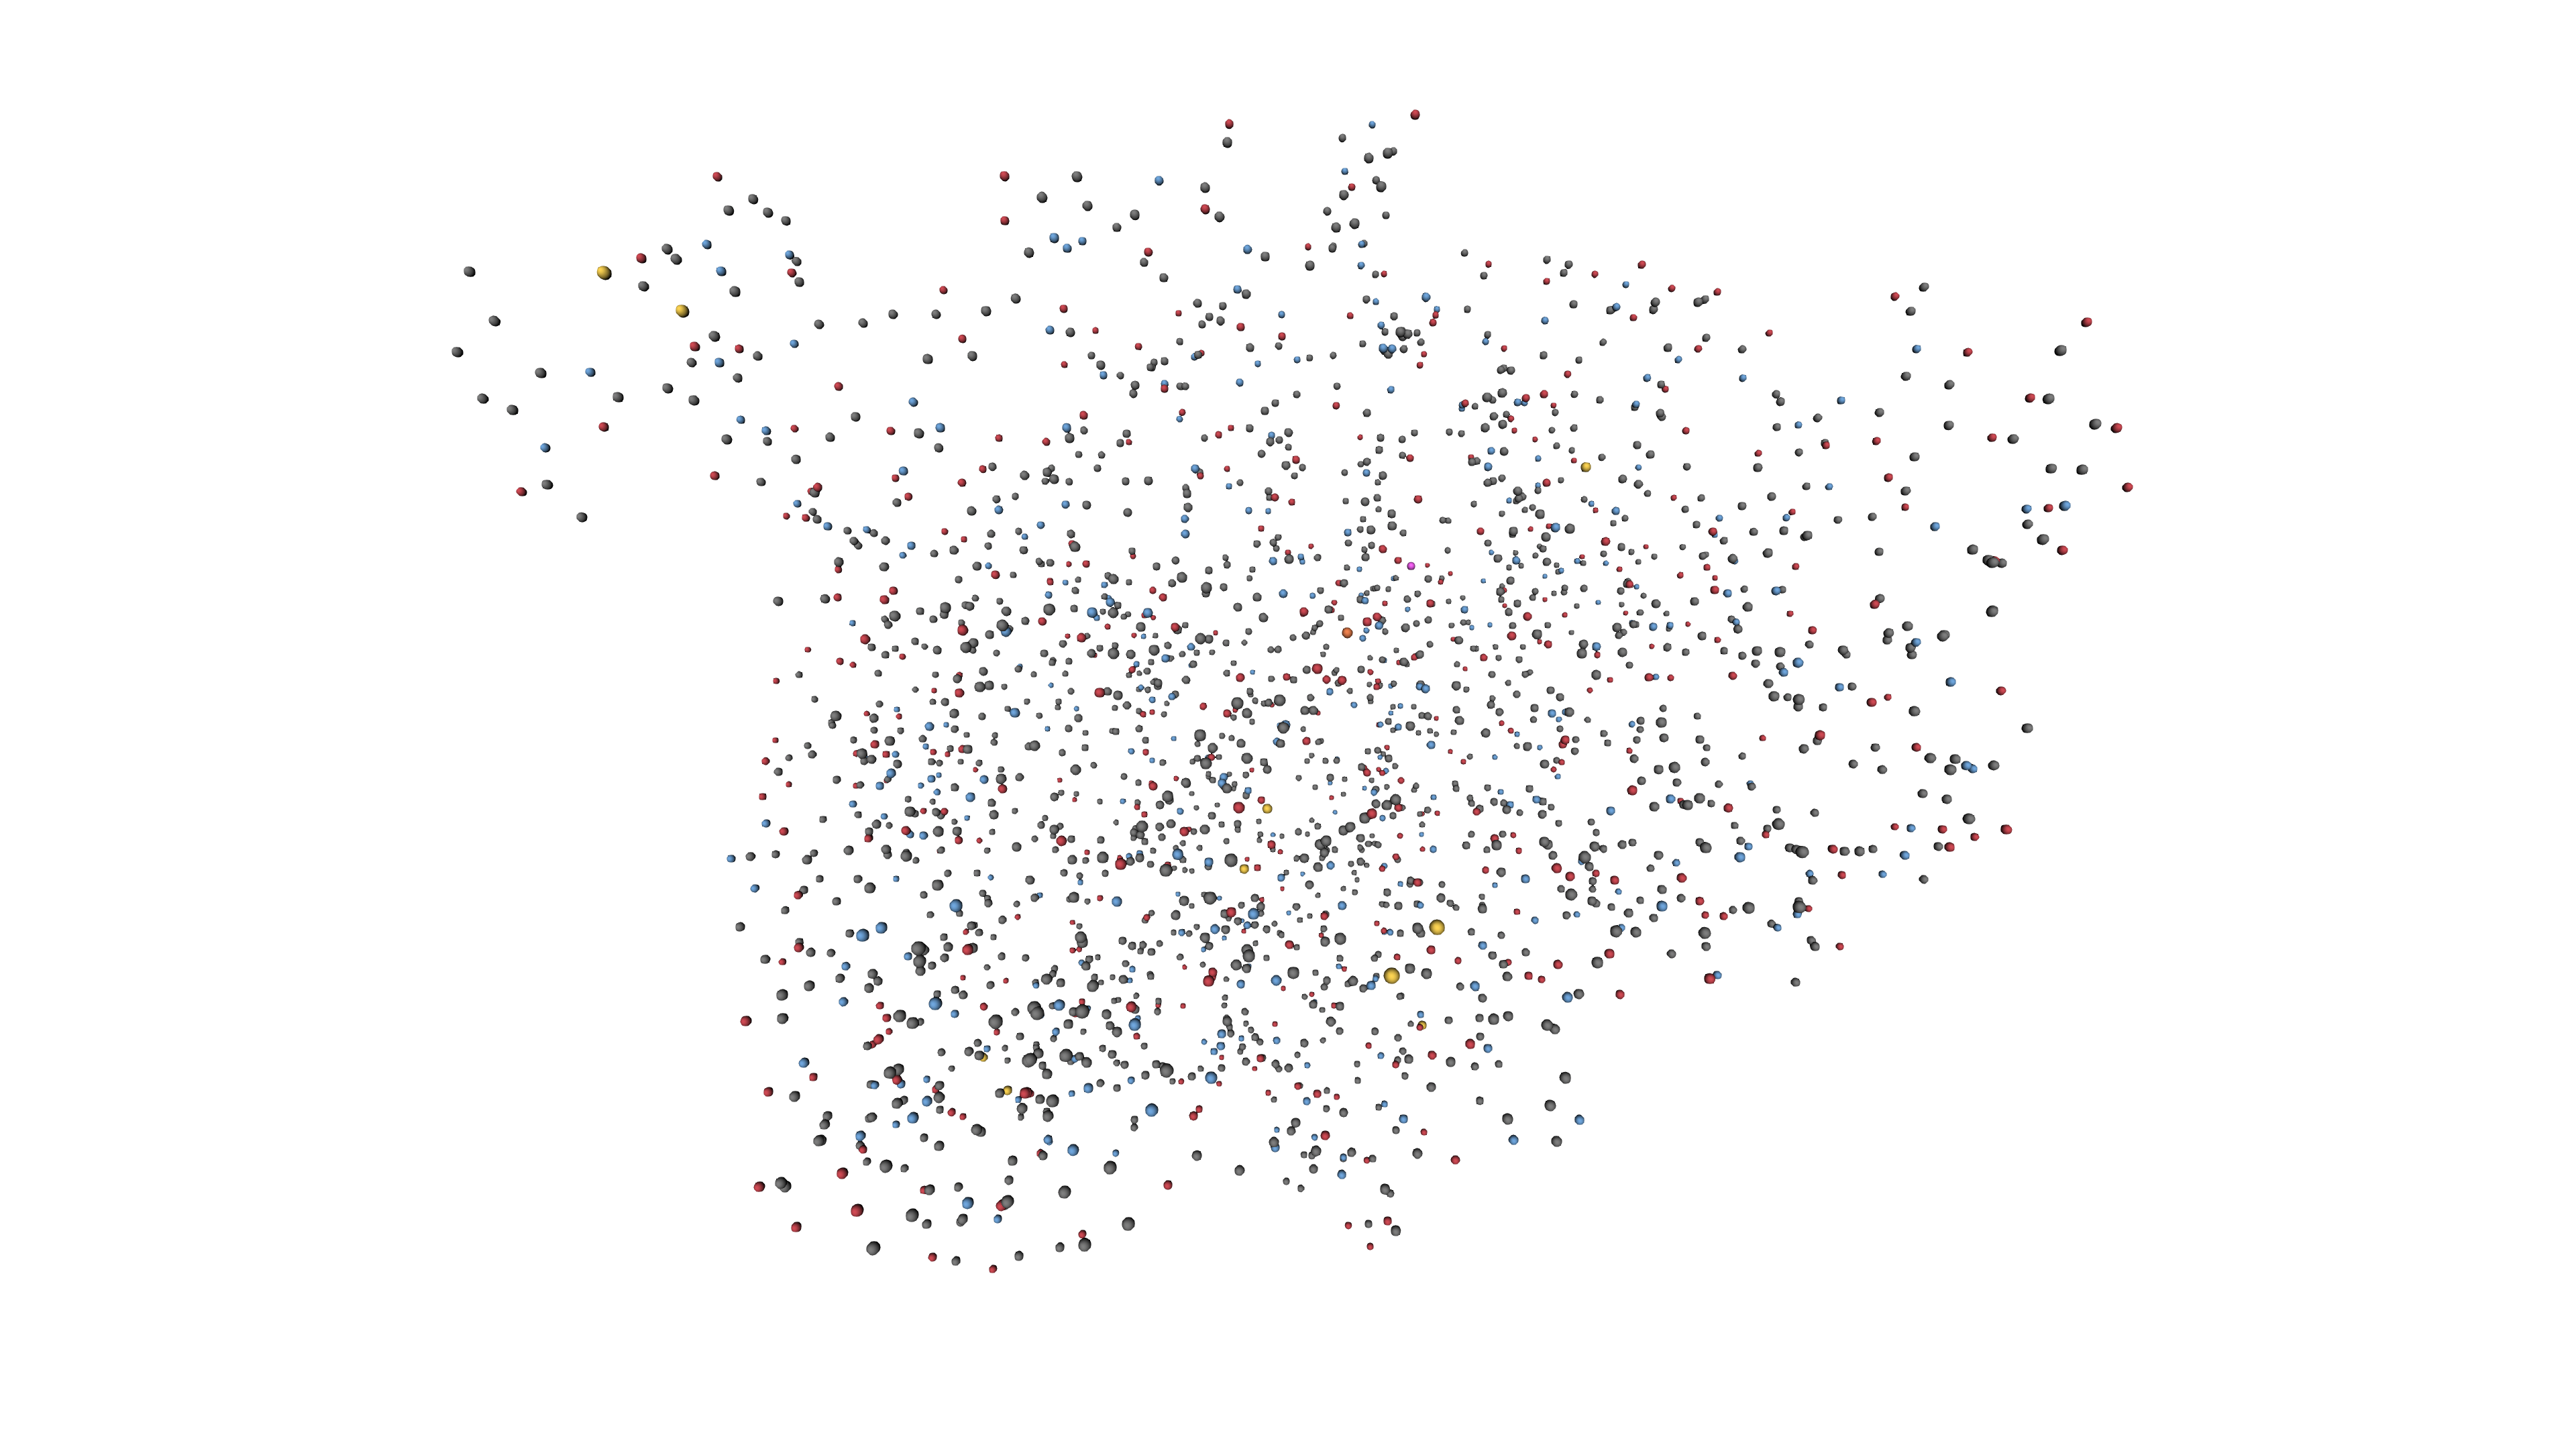
\includegraphics[width=\textwidth]{./figures/ch1/4awn_points}
			\caption[Représentation en points]{\textbf{Points :} seuls les atomes apparaissent.}
			\label{fig:4awn_points}
		\end{subfigure}
		~
		\begin{subfigure}[t]{\subImgW}
			\centering
			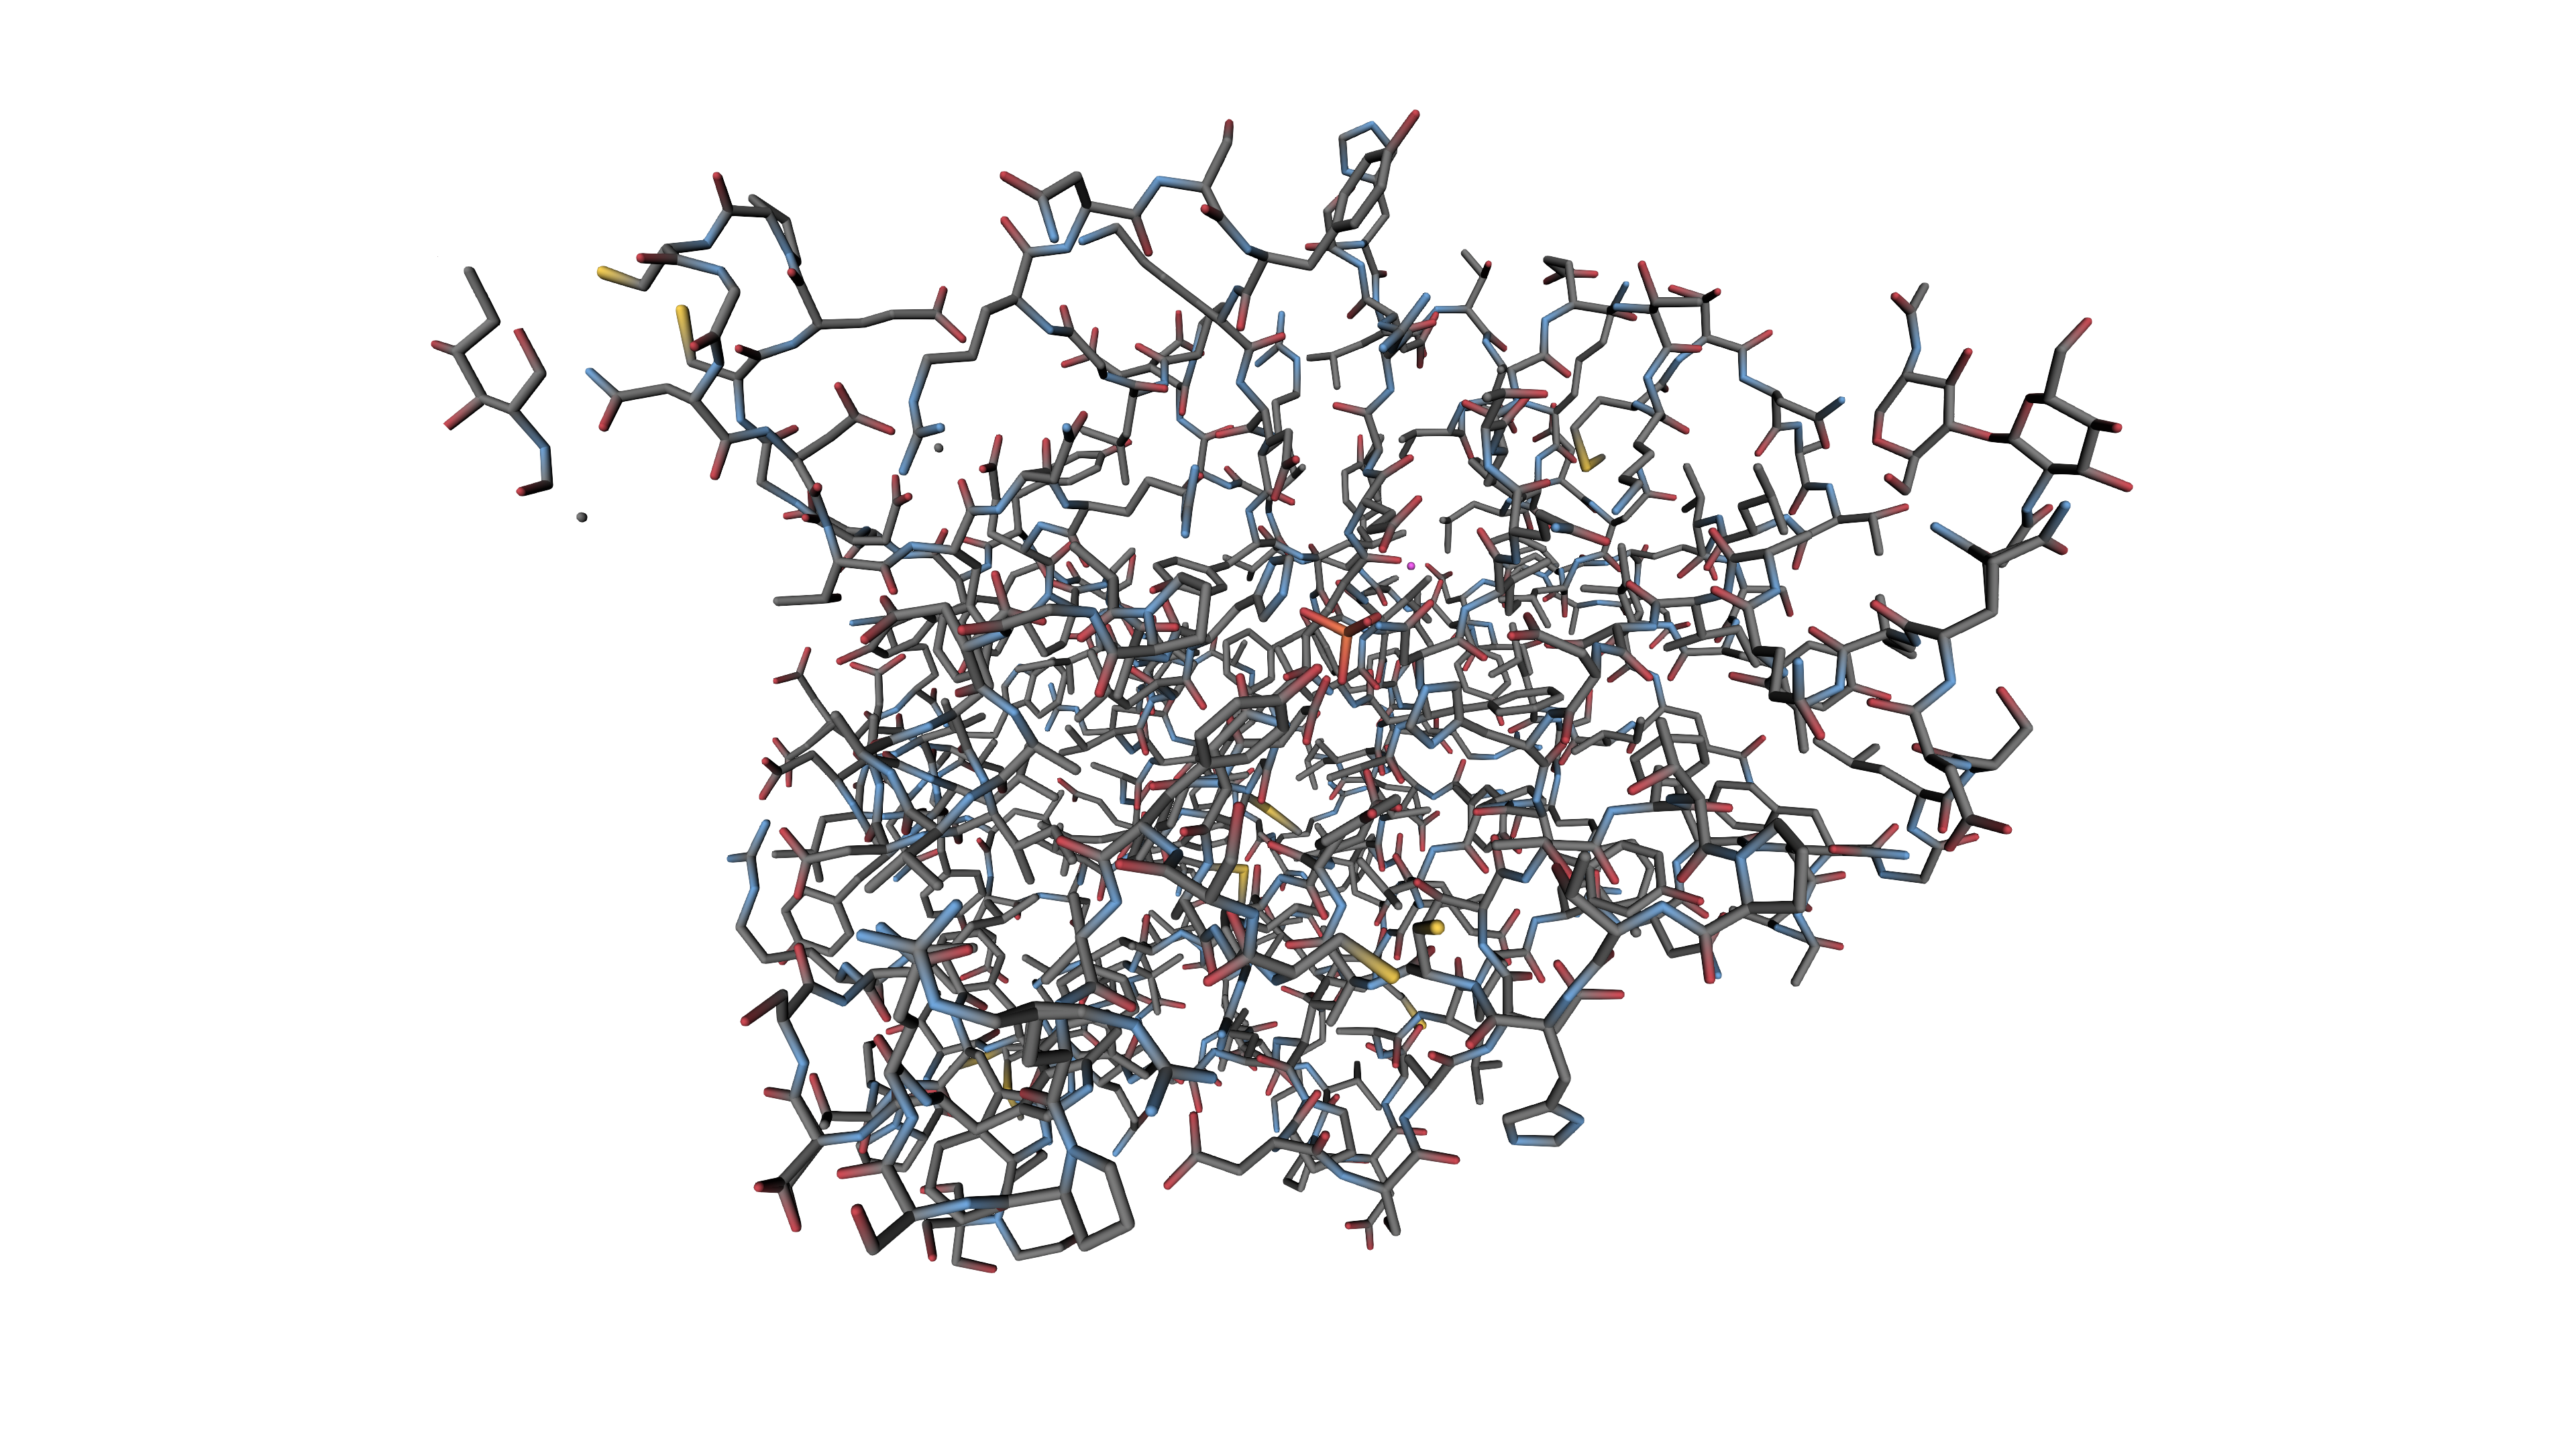
\includegraphics[width=\textwidth]{./figures/ch1/4awn_licorice}
			\caption[Représentation en réglisse]{\textbf{Bâtons, réglisse ou \emph{licorice} :} seules les liaisons covalentes sont visibles.}
			\label{fig:4awn_licorice}
		\end{subfigure}
		~
		\begin{subfigure}[t]{\subImgW}
			\centering
			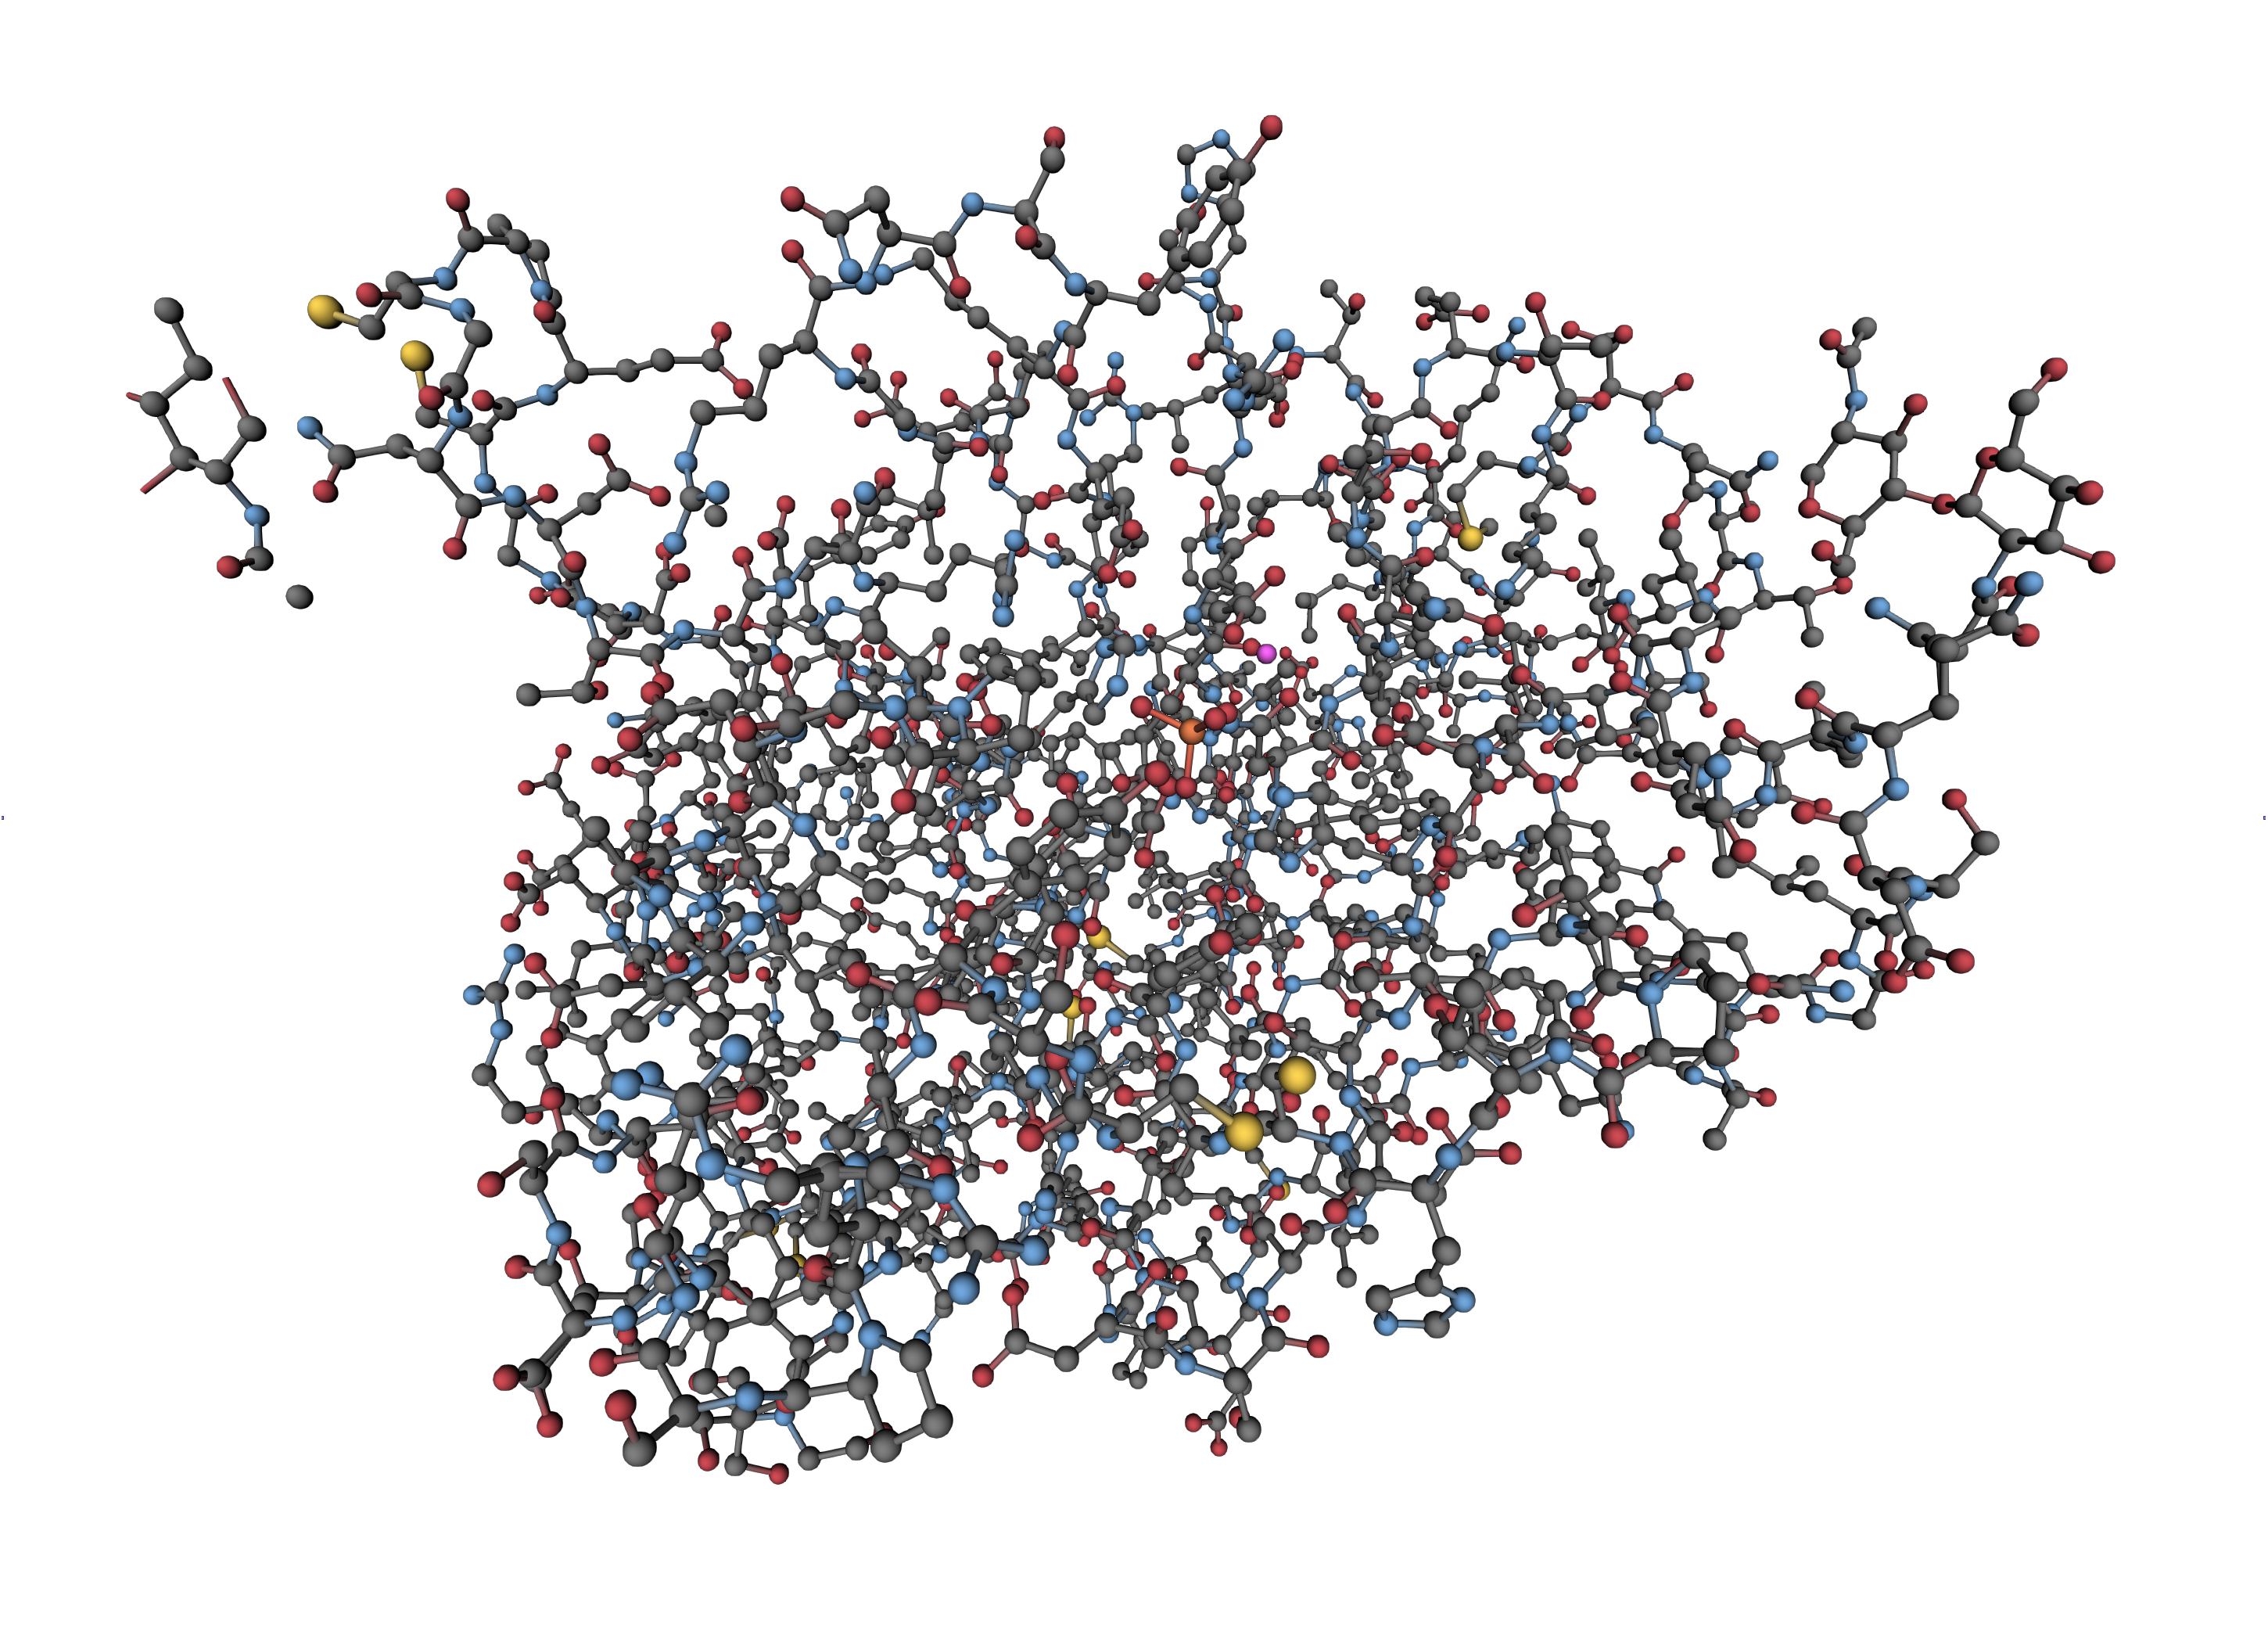
\includegraphics[width=\textwidth]{./figures/ch1/4awn_CPK}
			\caption[Représentation en CPK]{\textbf{CPK/boules et bâtons :} les atomes et les liaisons sont représentés.}
			\label{fig:4awn_CPK}
		\end{subfigure}
		~
		\begin{subfigure}[t]{\subImgW}
			\centering
			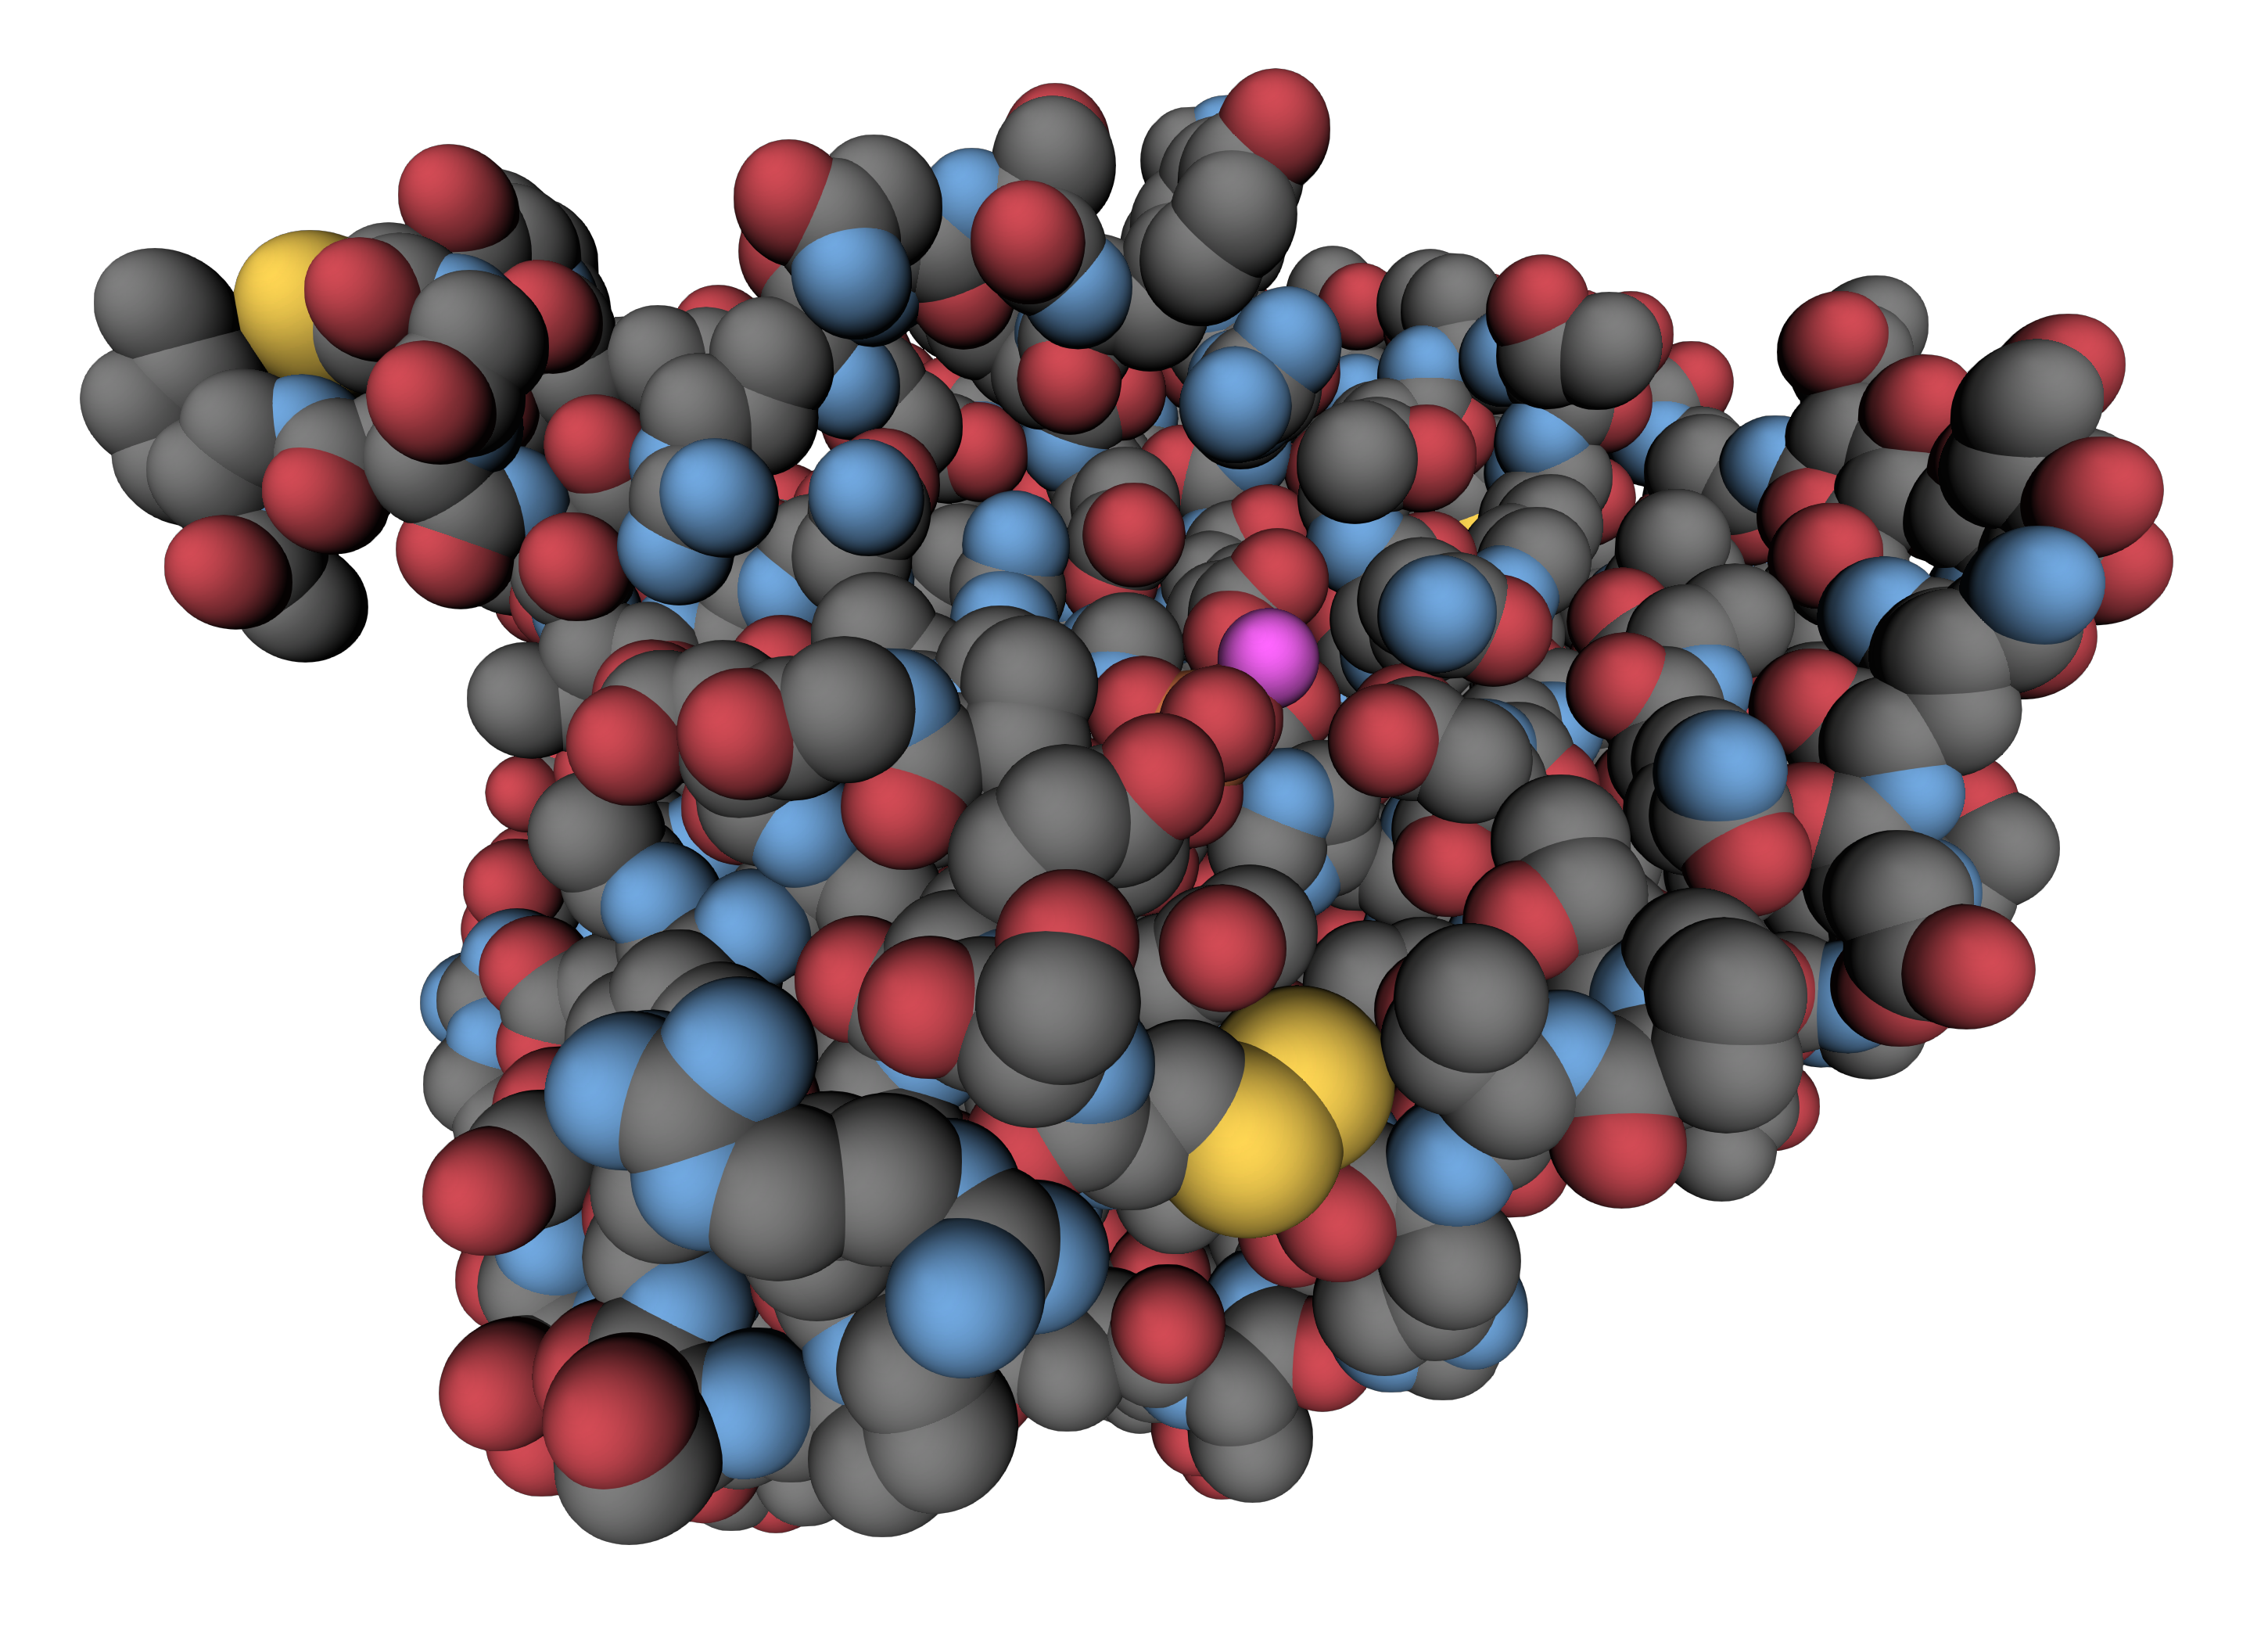
\includegraphics[width=\textwidth]{./figures/ch1/4awn_vdW}
			\caption[Représentation de van der Waals]{\textbf{Van der Waals :} seuls les atomes sont visibles.}
			\label{fig:4awn_VdW}
		\end{subfigure}
		~
		\begin{subfigure}[t]{\subImgW}
			\centering
			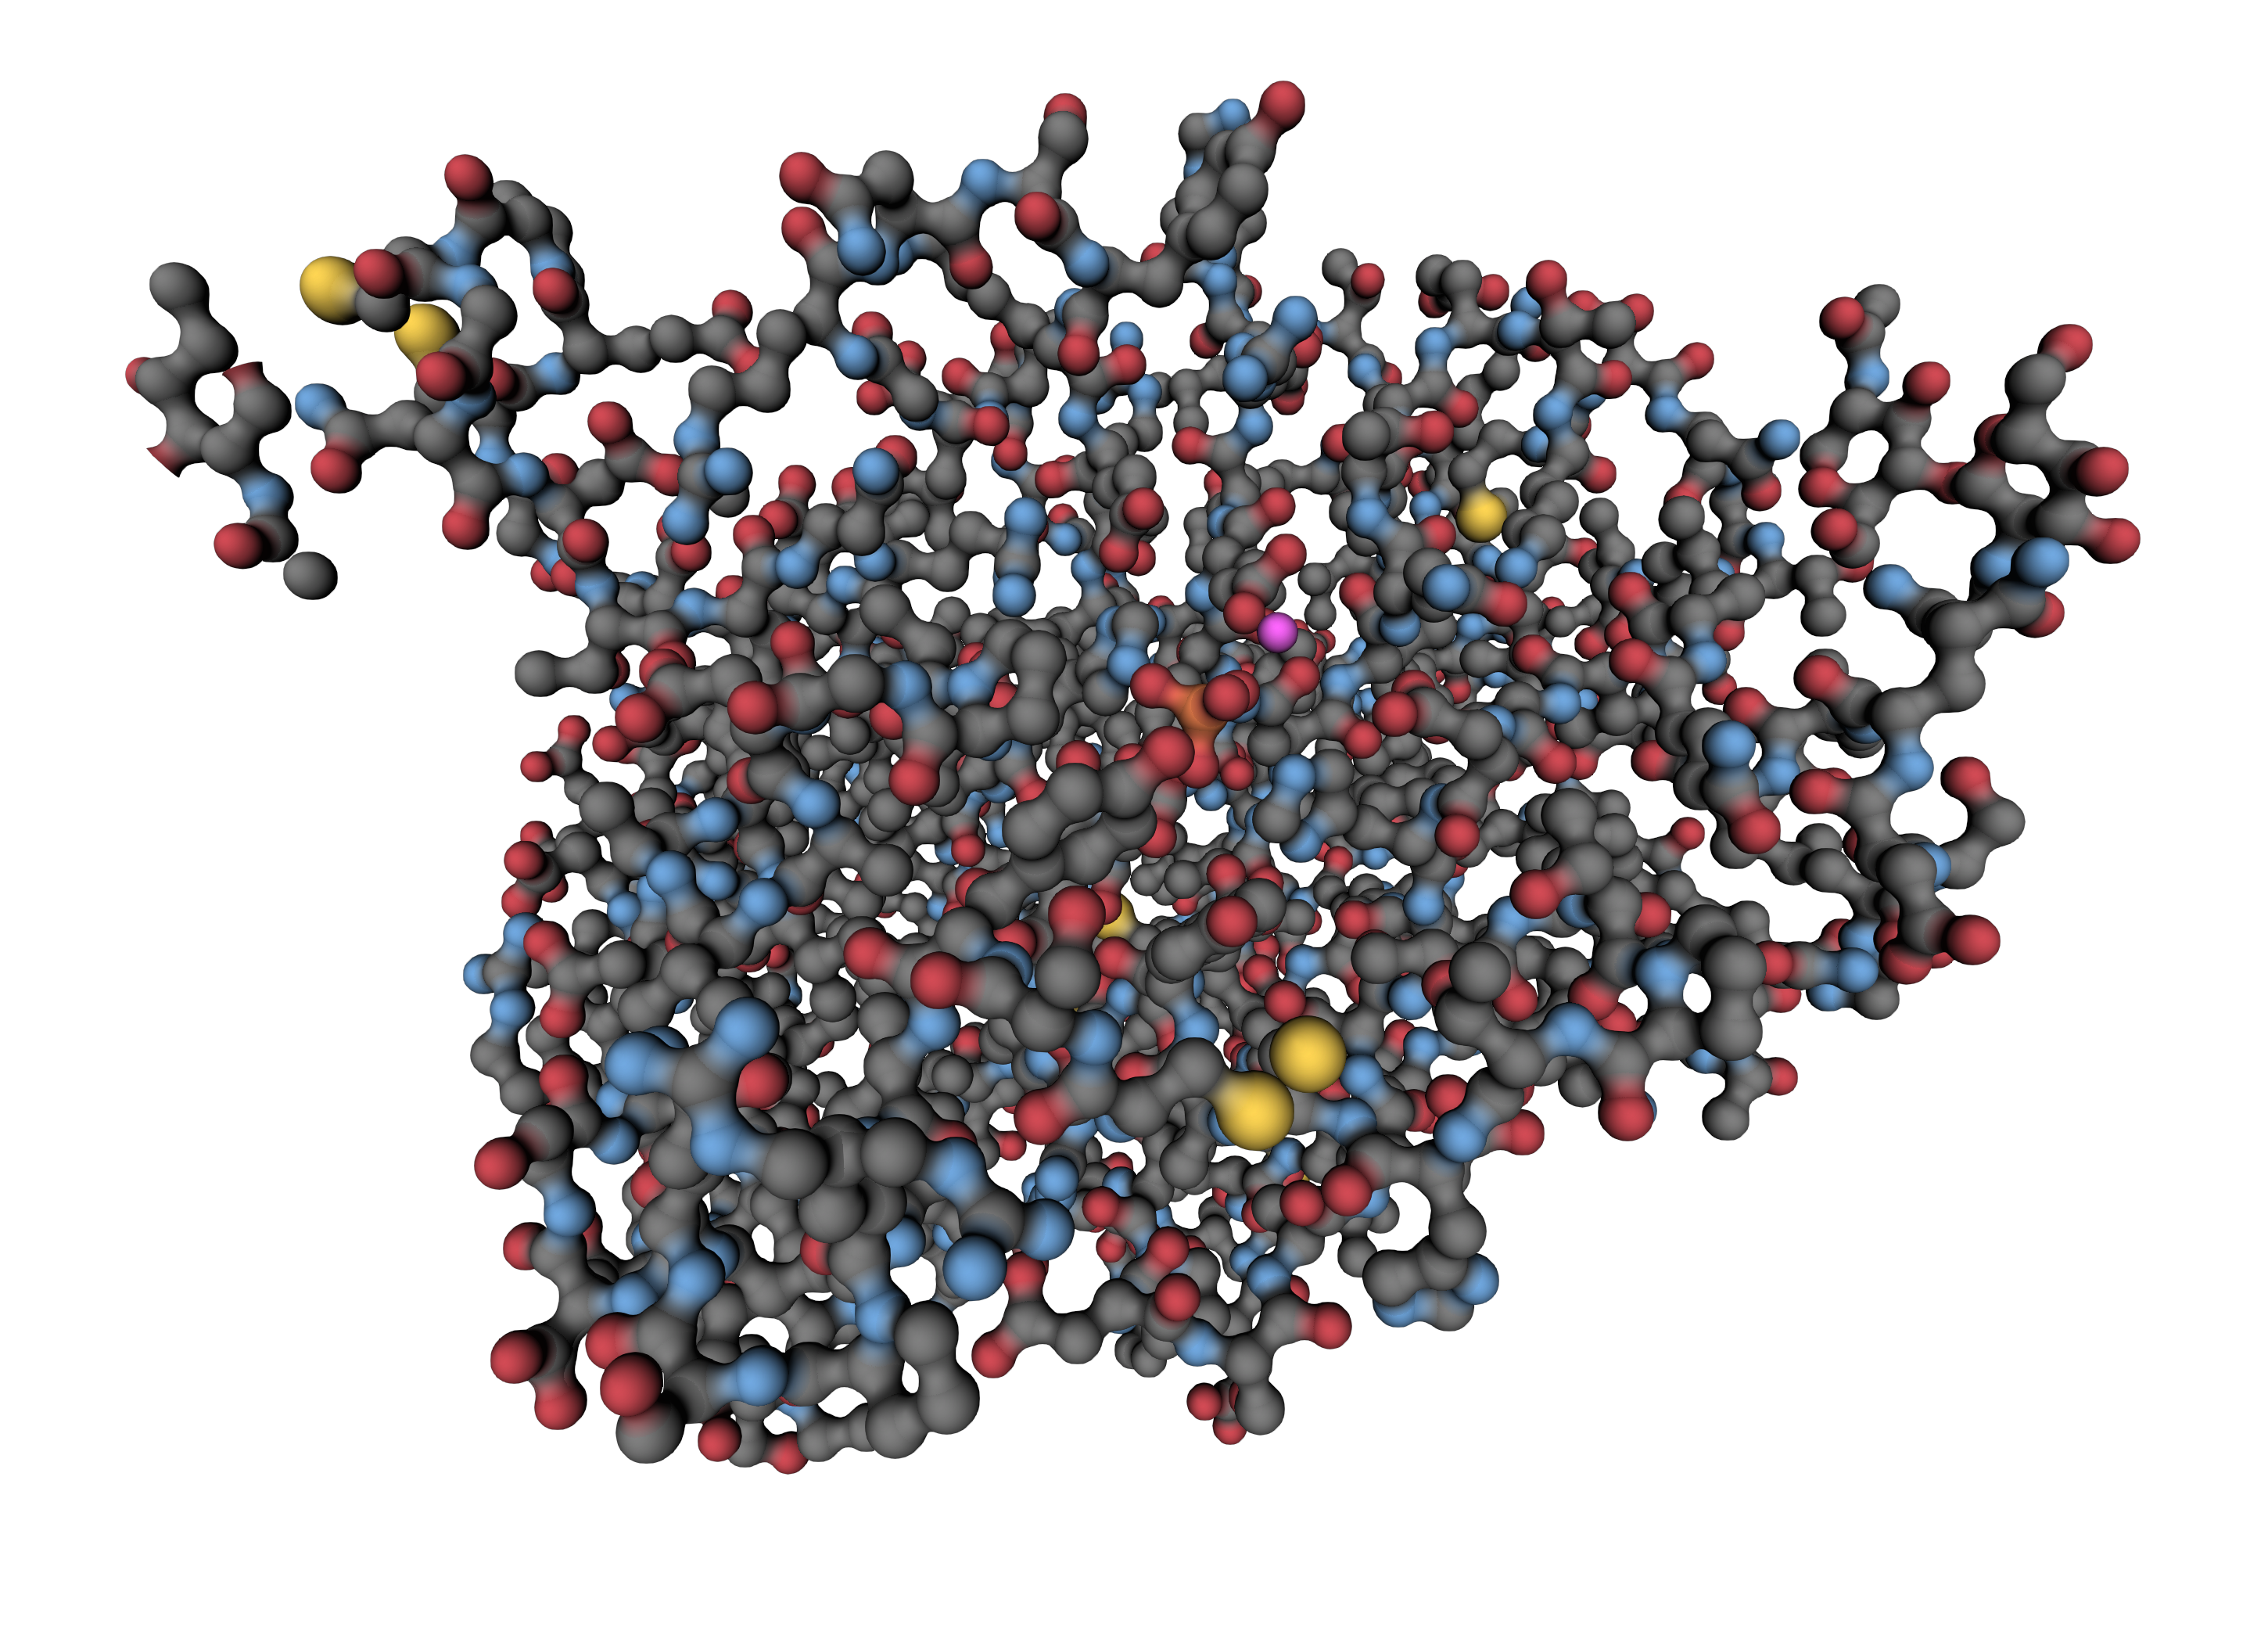
\includegraphics[width=\textwidth]{./figures/ch1/4awn_HB}
			\caption[Représentation en \emph{Hyperballs}]{\textbf{Hyperballs :} les atomes et les liaisons sont représentés~\cite{chavent2011gpu}.}
			\label{fig:4awn_HB}
		\end{subfigure}
		~
		\begin{subfigure}[t]{\subImgW}
			\centering
			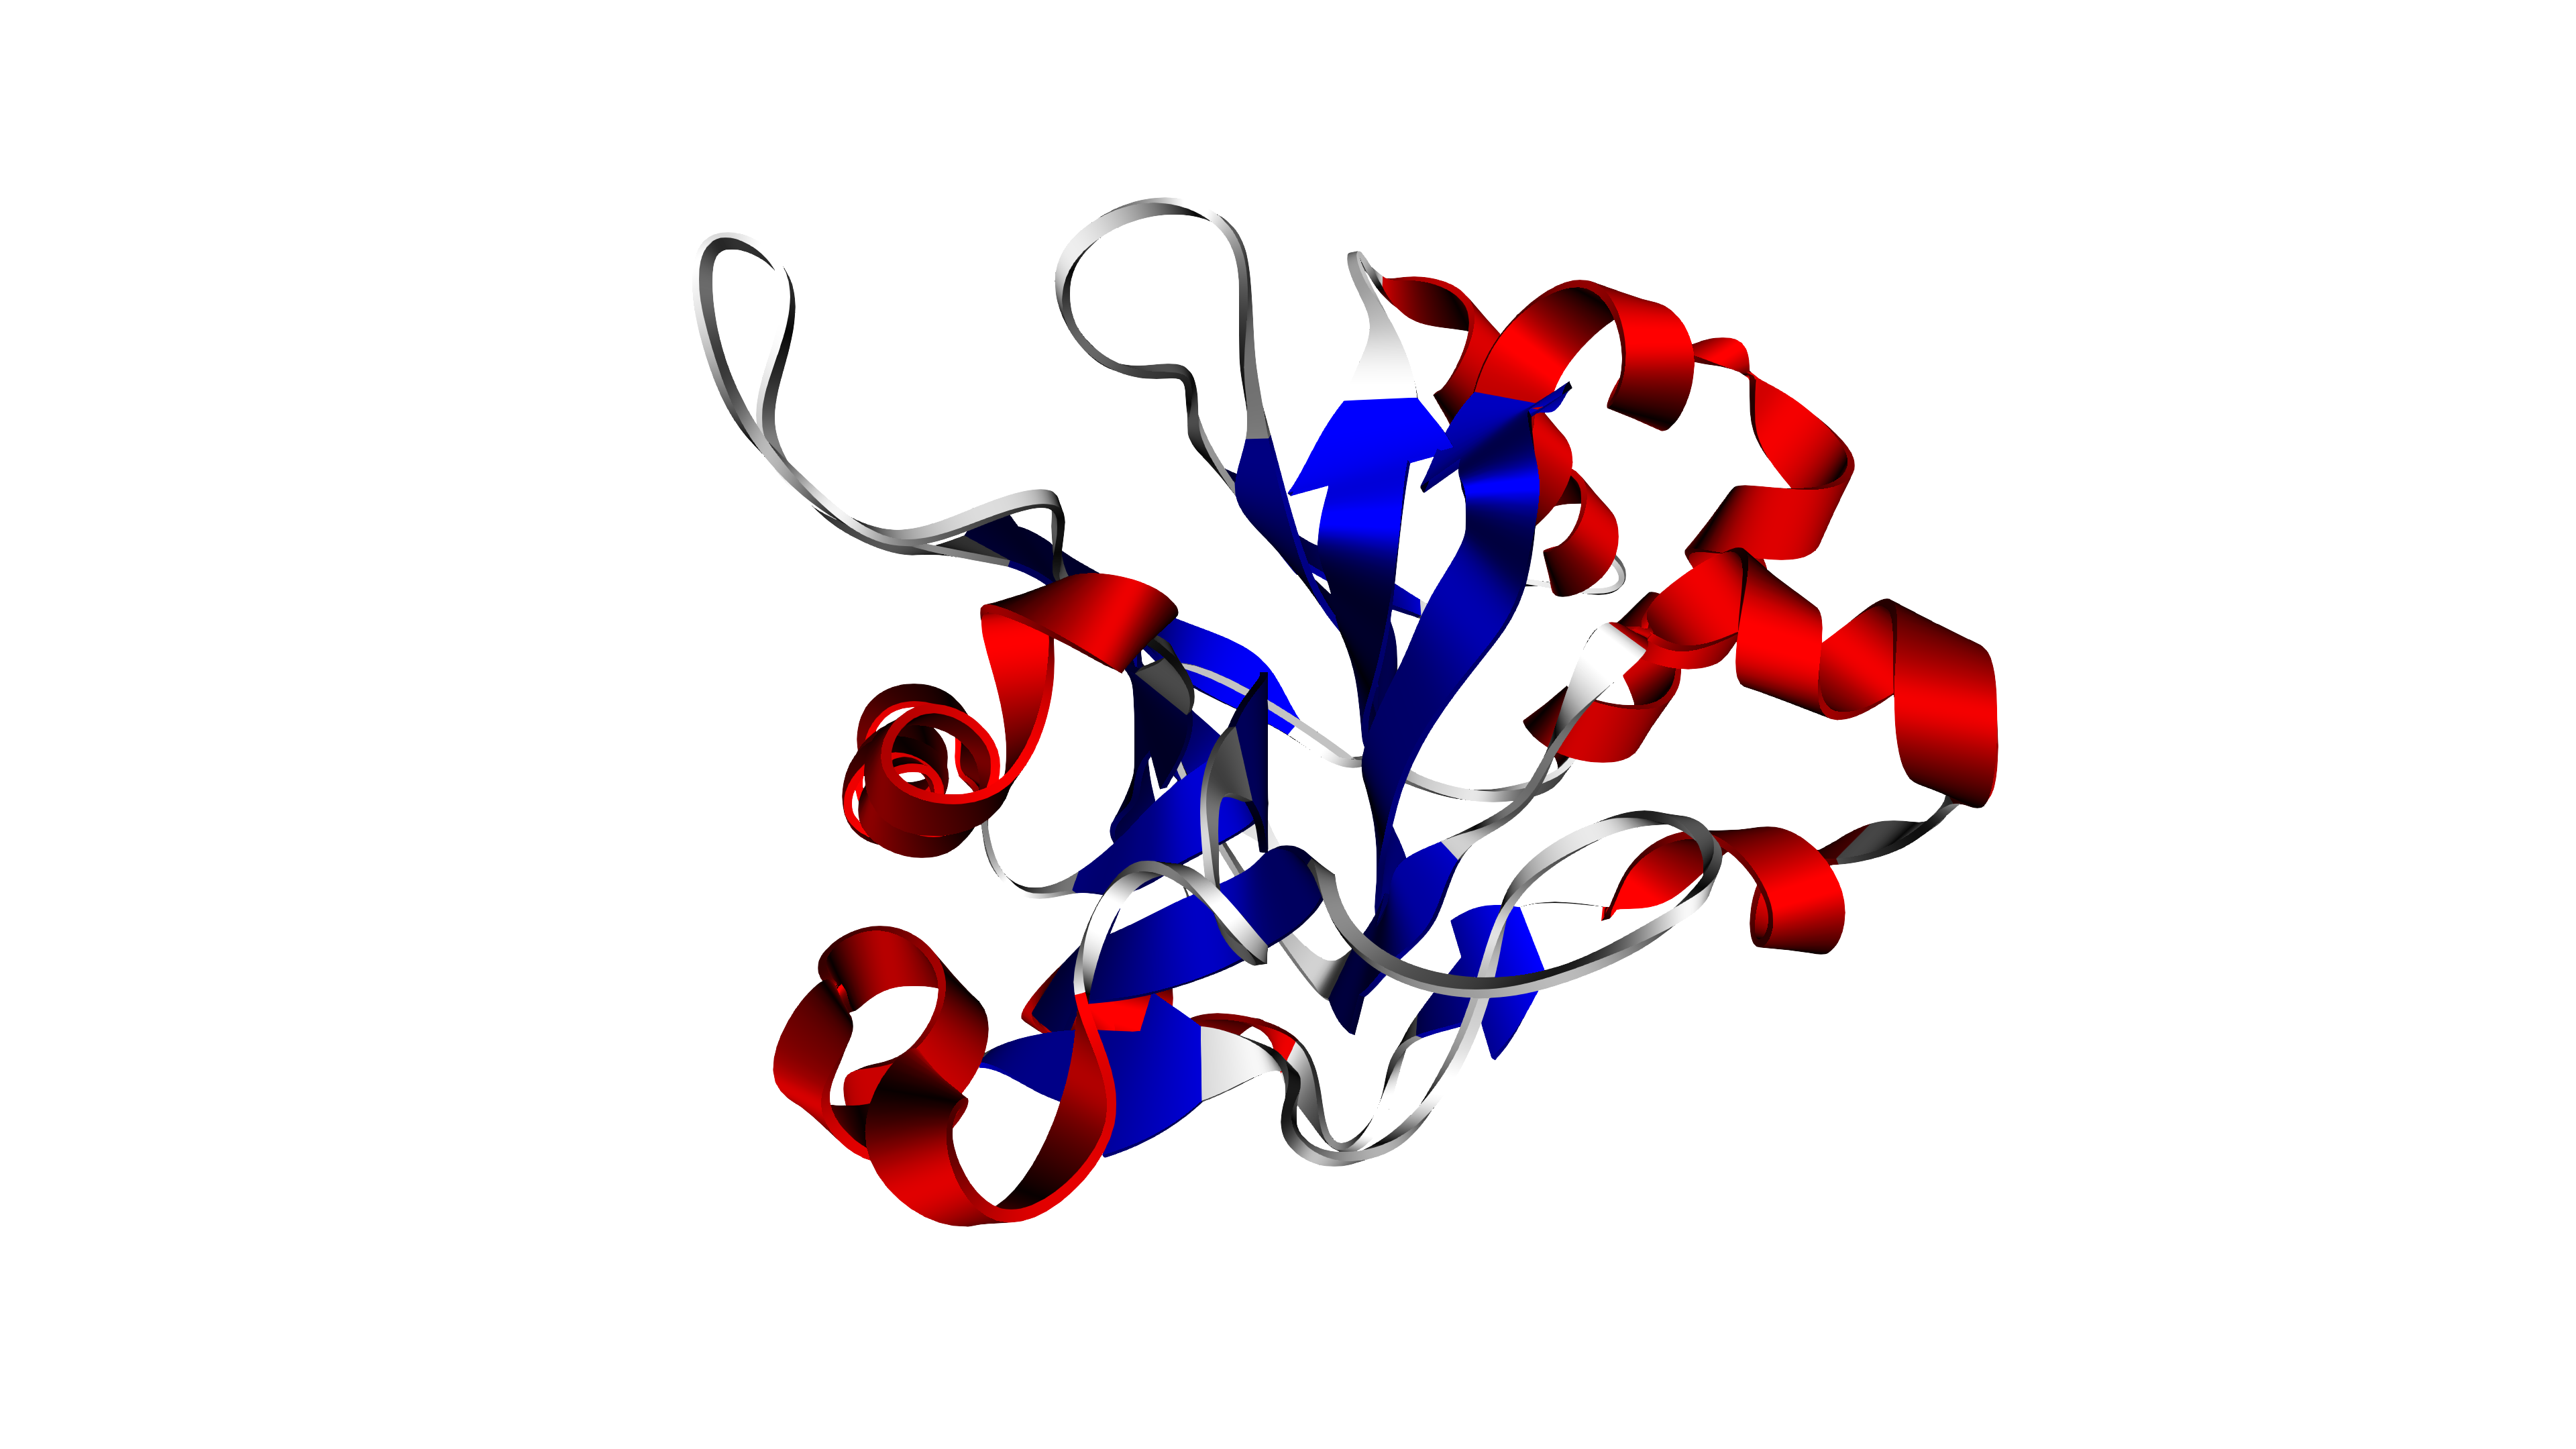
\includegraphics[width=\textwidth]{./figures/ch1/4awn_ss}
			\caption[Représentation en structures secondaires]{\textbf{Structures secondaires :} les atomes et les liaisons sont invisibles, mais des structures plus grandes sont représentées de façon schématique.}
			\label{fig:4awn_ss}
		\end{subfigure}
		~
		\begin{subfigure}[t]{\subImgW}
			\centering
			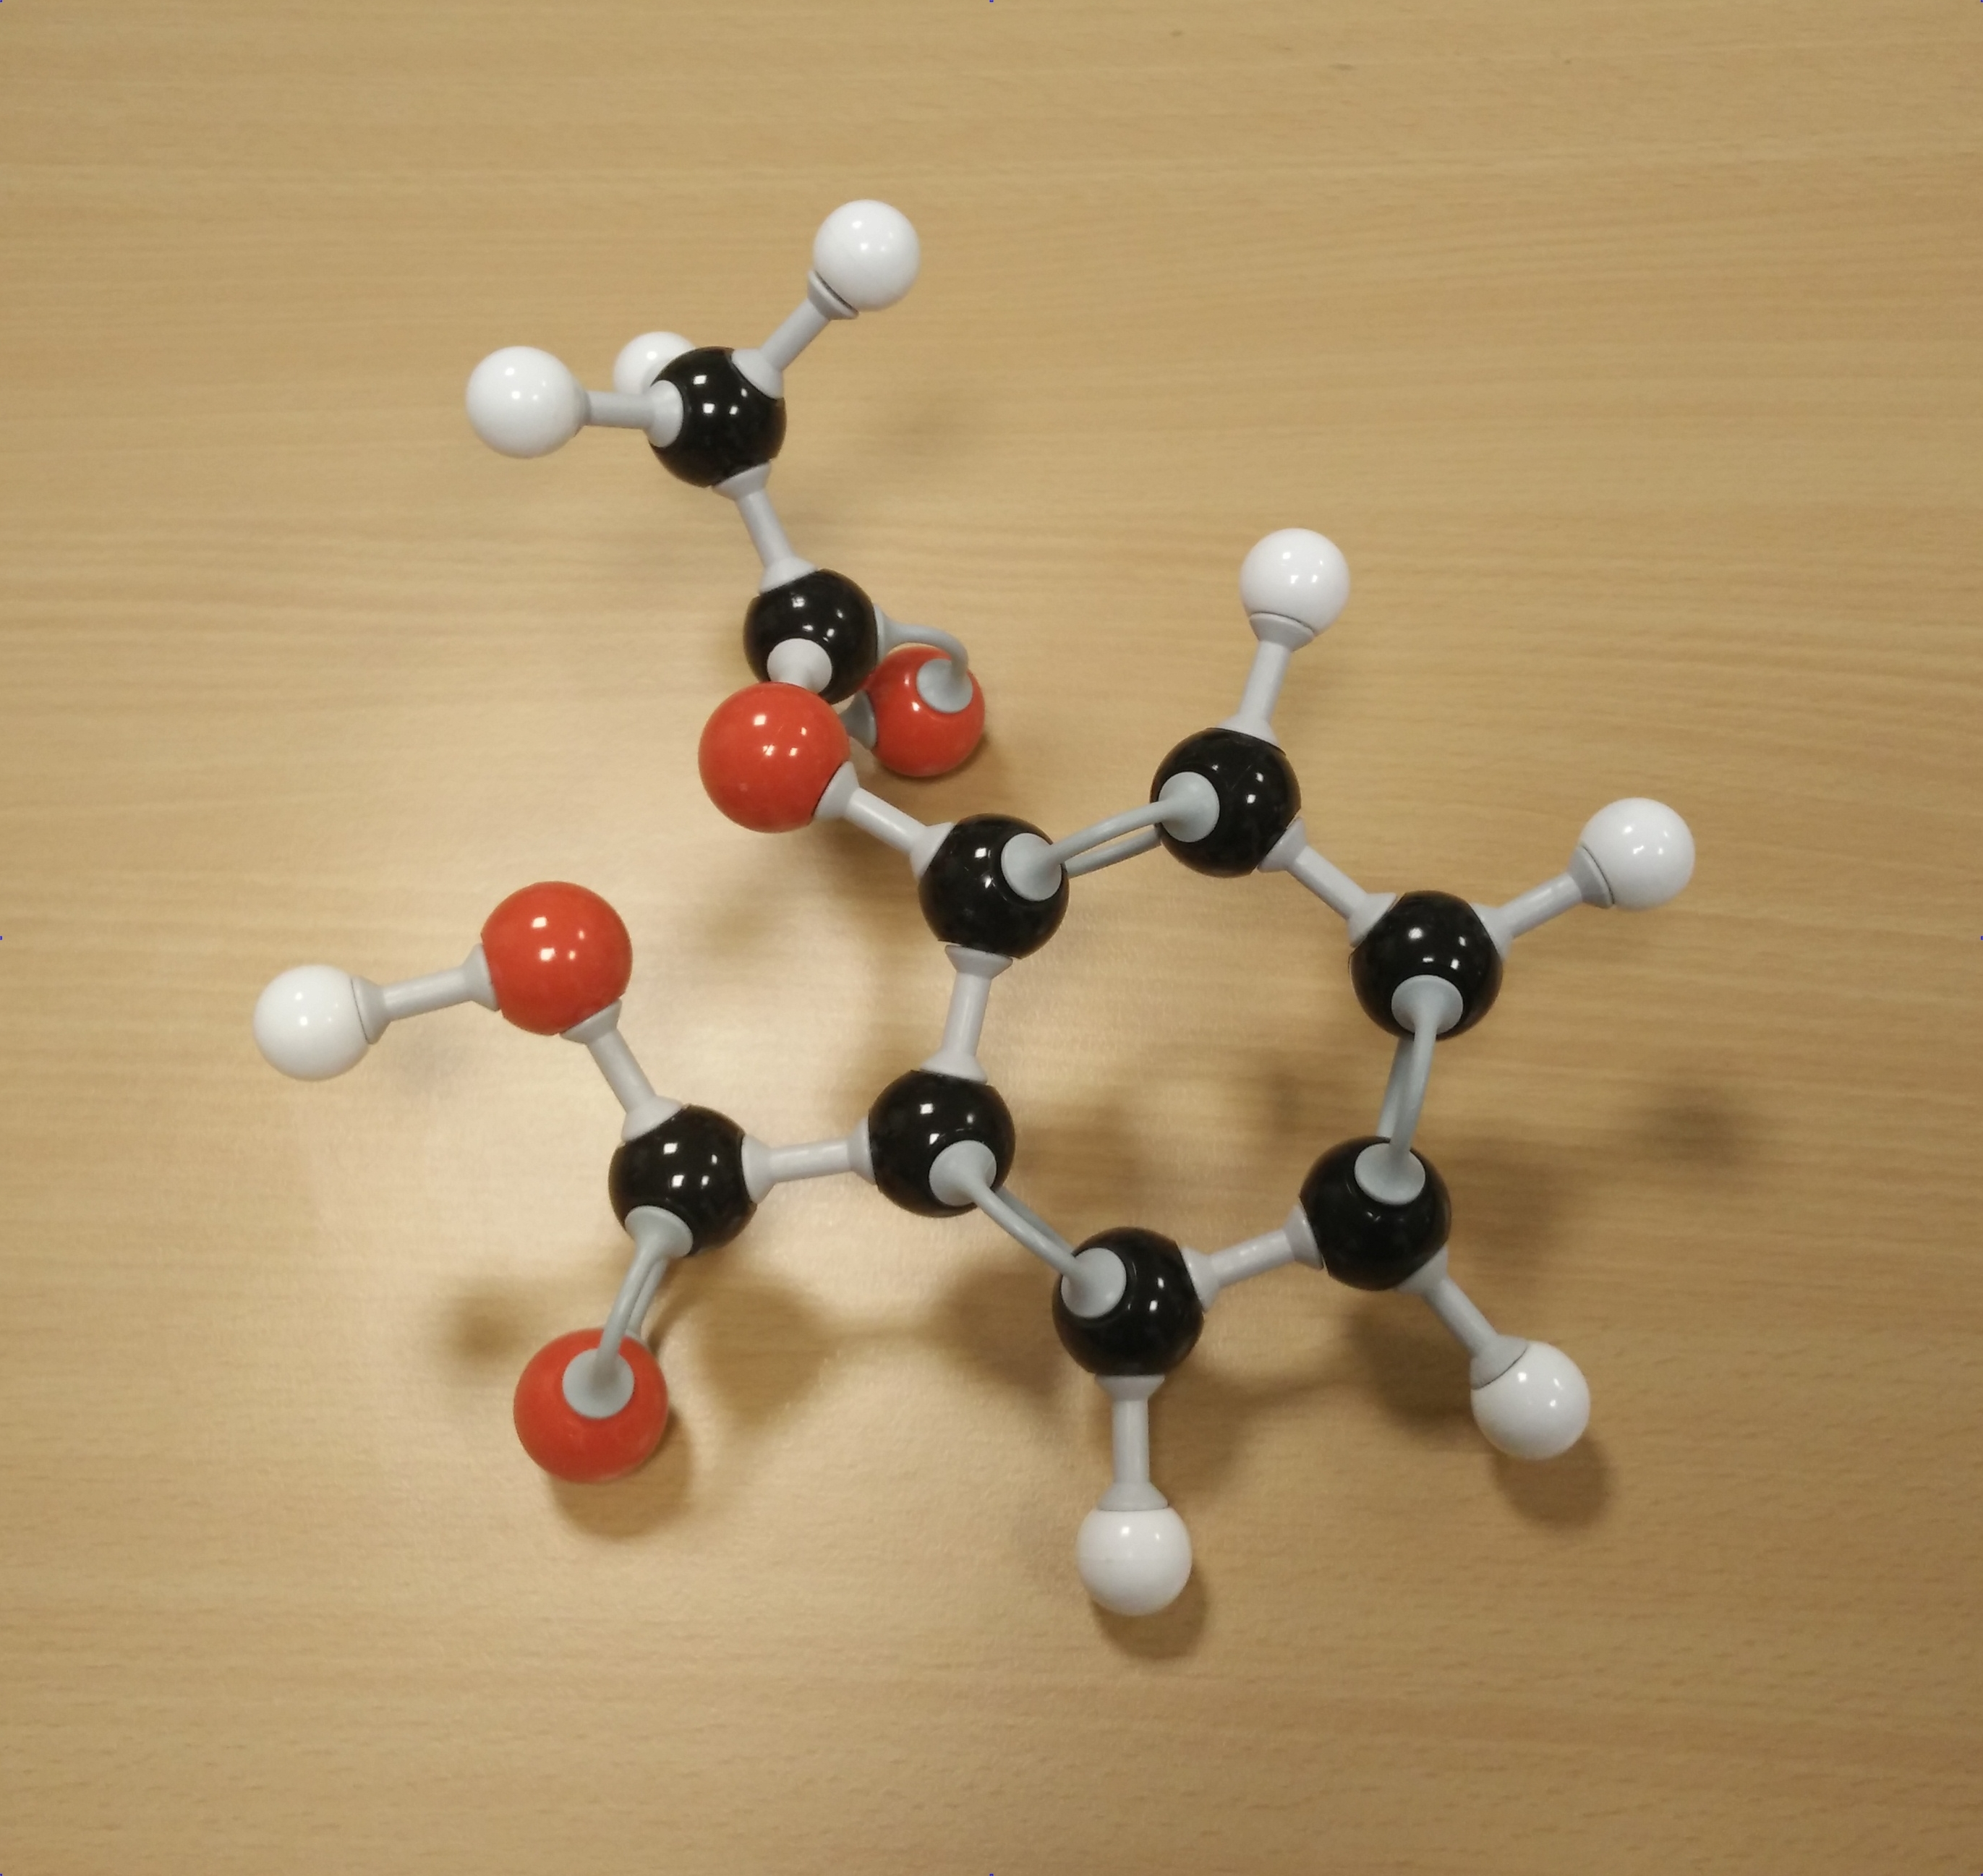
\includegraphics[width=\textwidth]{./figures/ch1/aspirin}
			\caption[Modèle physique de l'aspirine]{\textbf{Modèle physique }d'aspirine (et non d'ADNase). Les liaisons doubles sont modélisées par des paires de bâtons pour empêcher les rotations.}
			\label{fig:aspirin}
		\end{subfigure}
		~
		\begin{subfigure}[t]{\subImgW}
			\centering
			\includegraphics[width=\textwidth]{./figures/ch1/4awn_ses}
			\caption[Représentation en surface de Connolly]{\textbf{Surface de Connolly, ou \emph{solvent excluded surface} :} les points de contact entre une molécule d'eau et l'ADNase.}
			\label{fig:4awn_ses}
		\end{subfigure}
		~
		\begin{subfigure}[t]{\subImgW}
			\centering
			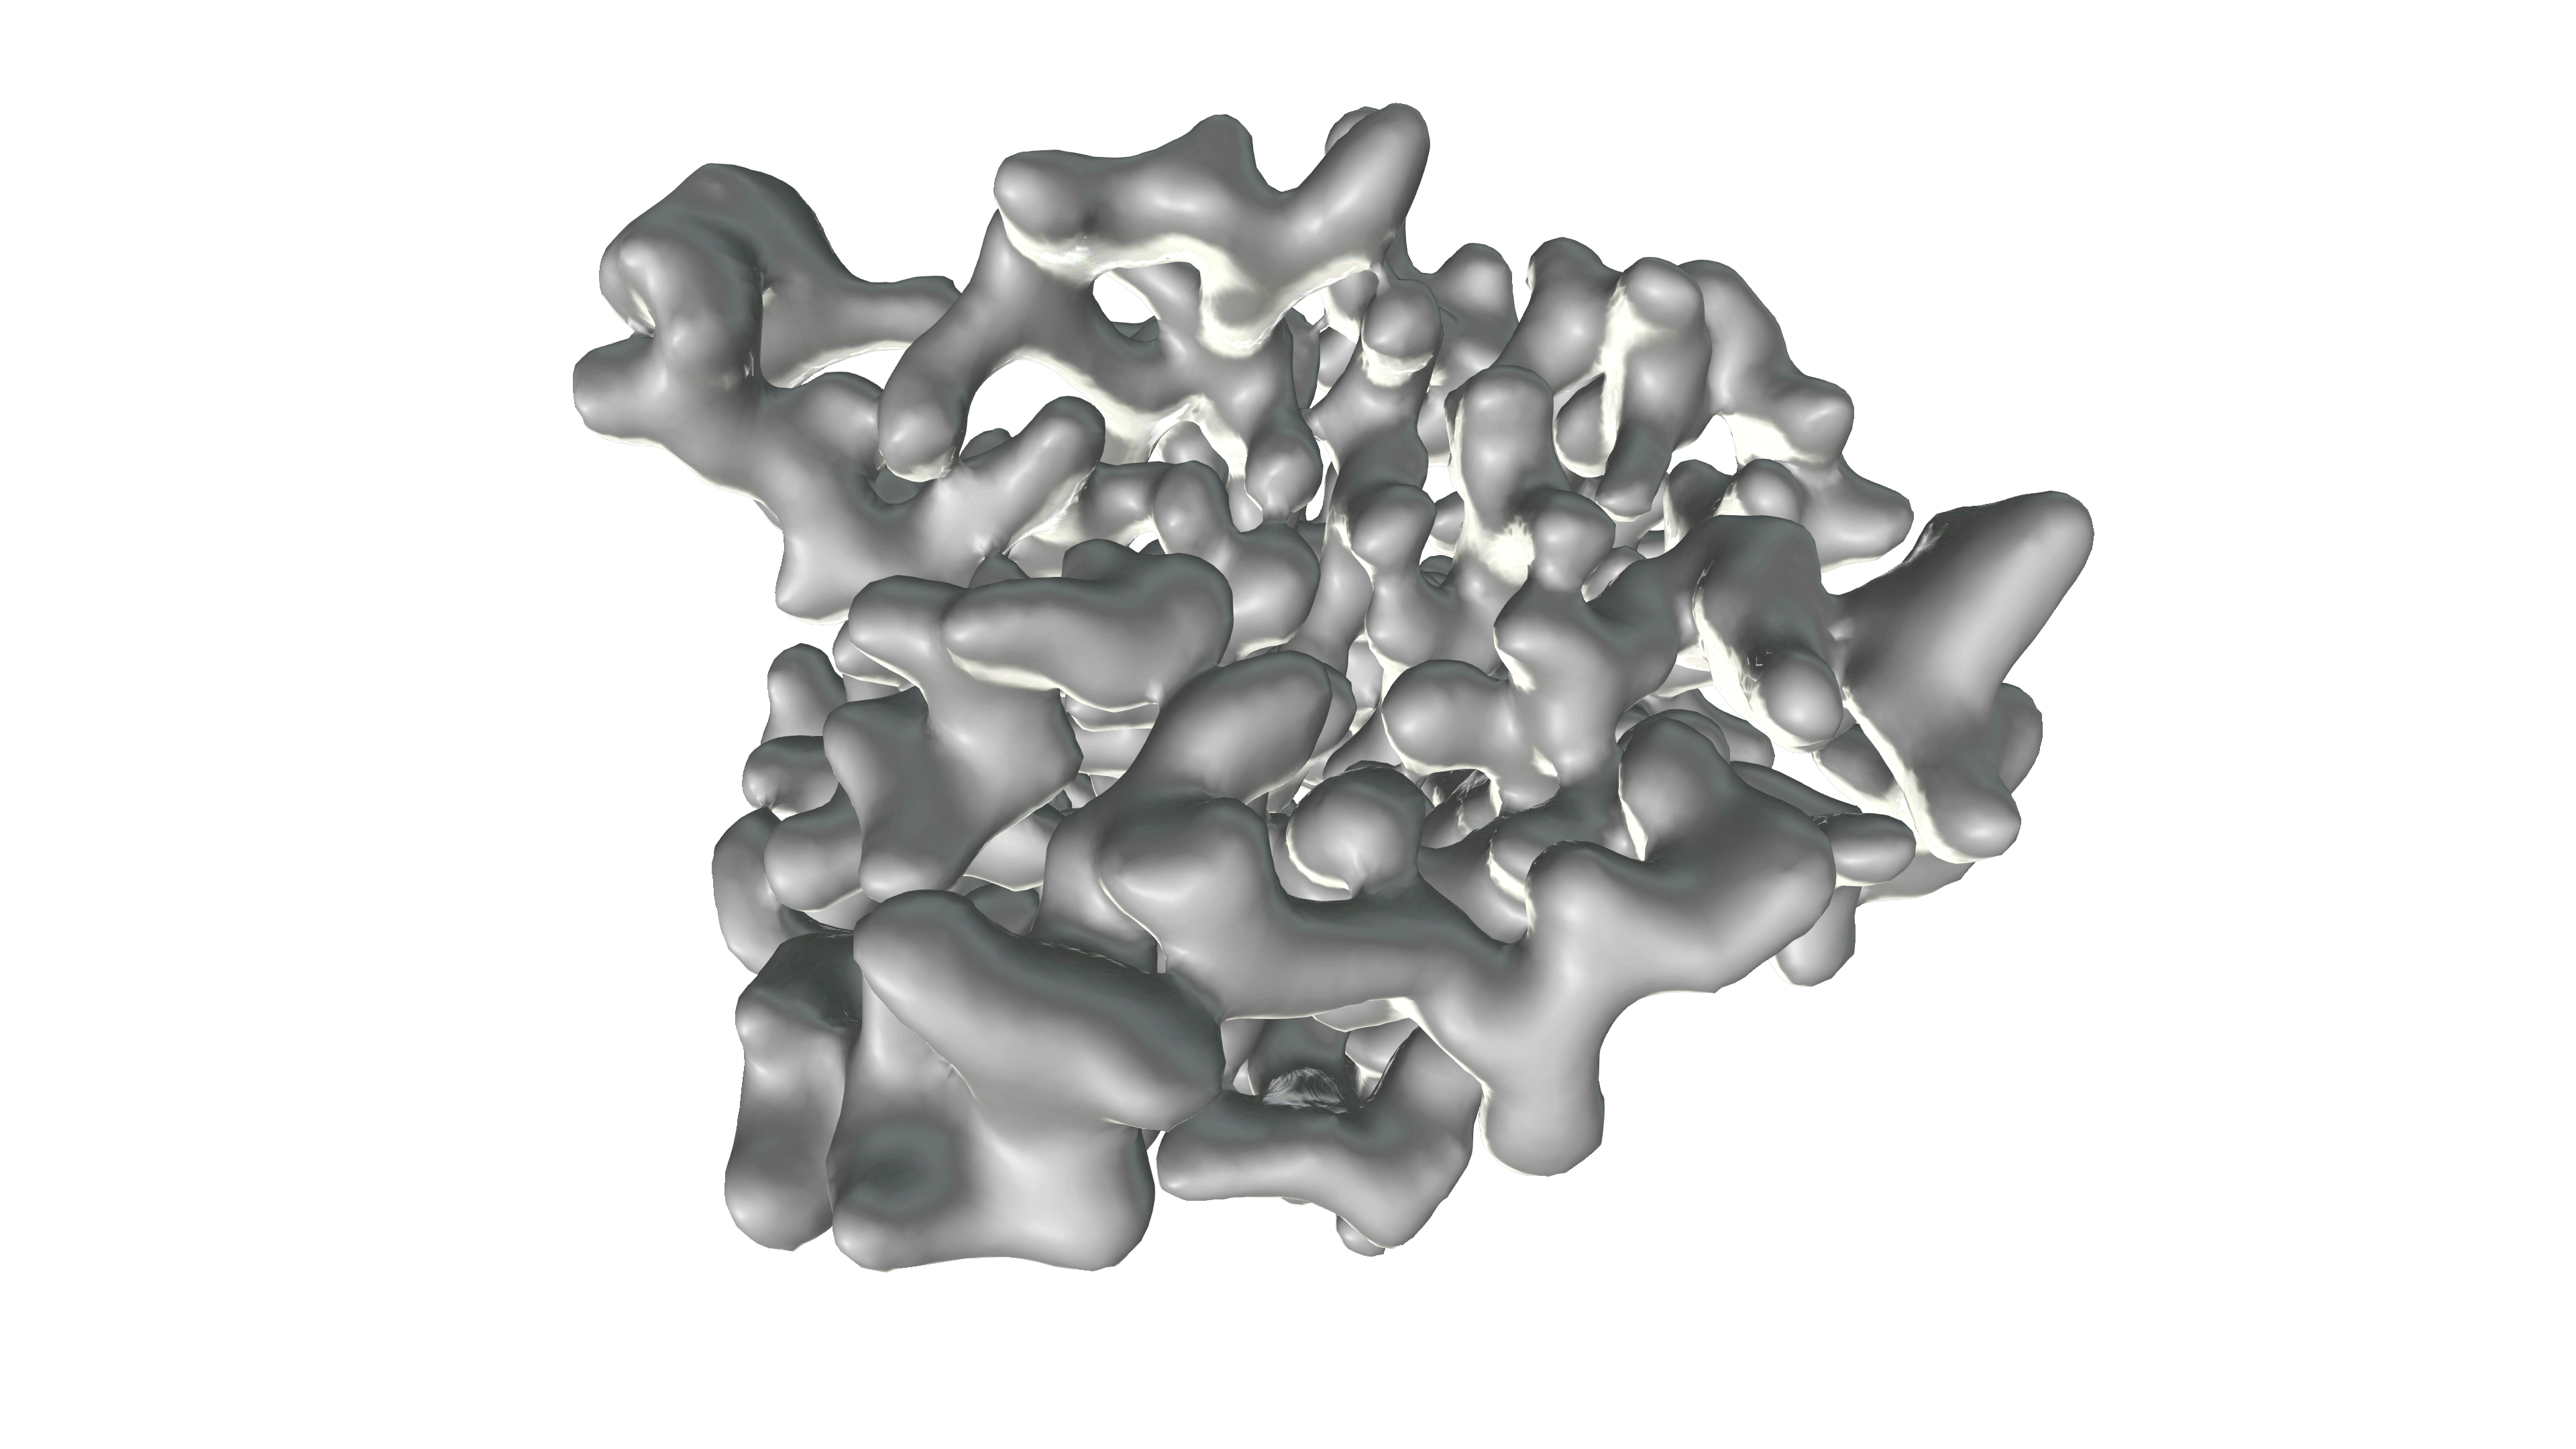
\includegraphics[width=\textwidth]{./figures/ch1/4awn_iso_1_5}
			\caption[Isosurface de densité]{\textbf{Isosurface de densité :} la surface est constituée des points de densité $1,5$.}
			\label{fig:4awn_iso_1_5}
		\end{subfigure}
		\caption[Modes de représentation moléculaire]{La désoxyribonucléase (ADNase) est une enzyme catalysant les acides désoxyribonucléiques en nucléotides ou polynucléotides. Voici quelques techniques de visualisation moléculaire, avec l'ADNase pour objet. Illustrations produites par \emph{UnityMol}~\cite{doutreligne2014unitymol} à partir d'une structure de la \emph{Protein Data Bank}~\cite{parsiegla2012structure}.}
		\label{fig:4awn_atom}
	\end{figure}